\makeoutercover
\makeinnercover

\pagenumbering{gobble}

\chapter*{THÔNG TIN HỘI ĐỒNG CHẤM KHÓA LUẬN TỐT NGHIỆP}

Hội đồng chấm khóa luận tốt nghiệp được thành lập theo Quyết định số:

\begin{center}
\ldots\ldots\ldots\ldots\ldots\ldots\ldots\ldots
\end{center}

Ngày \ldots\ldots/\ldots\ldots/\ldots\ldots{} của Hiệu trưởng Trường
Đại học Công nghệ Thông tin.

\clearpage
\chapter*{LỜI CẢM ƠN}

Lời đầu tiên, nhóm chúng em xin gửi lời cảm ơn chân thành đến giảng viên
hướng dẫn, cô ThS. Trần Thị Hồng Yến thuộc Khoa Công nghệ Phần mềm,
Trường Đại học Công nghệ Thông tin -- Đại học Quốc gia TP.HCM, đã dành
thời gian hướng dẫn, xem xét và đóng góp ý kiến cho đề tài ``Xây dựng
mạng xã hội thông minh: Tích hợp AI kiểm duyệt và cá nhân hóa nội dung''.

Đề tài được thực hiện với mục tiêu phát triển một nền tảng mạng xã hội
đáp ứng nhu cầu kết nối, giao tiếp và chia sẻ thông tin. Trong quá trình
thực hiện, nhóm đã nghiên cứu và phân tích yêu cầu, thiết kế giao diện,
phát triển các chức năng mạng xã hội, xây dựng cơ chế cá nhân hóa nội
dung, giải thích thuật ngữ văn hóa mạng, nhắn tin, thông báo và hoàn
thiện hệ thống.

Mặc dù nhóm đã nỗ lực hoàn thành đề tài, báo cáo khó tránh khỏi những
hạn chế do phạm vi kiến thức và thời gian thực hiện. Nhóm rất mong nhận
được những ý kiến đóng góp quý báu của Quý Thầy/Cô để tiếp tục hoàn
thiện sản phẩm và nâng cao kiến thức chuyên môn.

\vspace{1.2cm}
\begin{flushright}
Xin chân thành cảm ơn Quý Thầy/Cô!\par
\vspace{0.25cm}
Nhóm sinh viên thực hiện:\par
\vspace{1.4cm}
\textbf{Gia Bảo Anh}\par
\textbf{Nguyễn Thị Như Huỳnh}
\end{flushright}

\clearpage
\pagenumbering{roman}
\setcounter{page}{1}
\tableofcontents
\clearpage
\listoffigures
\clearpage
\listoftables
\clearpage

\chapter*{DANH MỤC TỪ VIẾT TẮT}
\addcontentsline{toc}{chapter}{DANH MỤC TỪ VIẾT TẮT}

{\def\LTcaptype{none} % do not increment counter
\begin{longtable}[]{@{}
  >{\centering\arraybackslash}p{(\linewidth - 6\tabcolsep) * \real{0.0955}}
  >{\centering\arraybackslash}p{(\linewidth - 6\tabcolsep) * \real{0.1450}}
  >{\centering\arraybackslash}p{(\linewidth - 6\tabcolsep) * \real{0.3860}}
  >{\centering\arraybackslash}p{(\linewidth - 6\tabcolsep) * \real{0.3517}}@{}}
\toprule\noalign{}
\endhead
\bottomrule\noalign{}
\endlastfoot
\textbf{STT} & \textbf{Ký hiệu} & \textbf{Tiếng Anh} & \textbf{Tiếng
Việt} \\
1 & AI & Artificial Intelligence & Trí tuệ nhân tạo \\
2 & API & Application Programming Interface & Giao diện lập trình ứng
dụng \\
3 & UI & User Interface & Giao diện người dùng \\
4 & UX & User Experience & Trải nghiệm người dùng \\
5 & 2FA & Two-Factor Authentication & Xác thực hai yếu tố \\
6 & LLM & Large Language Model & Mô hình ngôn ngữ lớn \\
7 & CTR & Click-Through Rate & Tỉ lệ nhấp \\
8 & NLP & Natural Language Processing & Xử lý ngôn ngữ tự nhiên \\
9 & MVP & Minimum Viable Product & Sản phẩm khả dụng tối thiểu \\
10 & REST & Representational State Transfer & Kiểu kiến trúc truyền tải
trạng thái đại diện \\
11 & ERD & Entity Relationship Diagram & Sơ đồ thực thể quan hệ \\
12 & SSR & Server-Side Rendering & Kết xuất phía máy chủ \\
13 & SSG & Static Site Generation & Tạo trang tĩnh \\
14 & CDN & Content Delivery Network & Mạng phân phối nội dung \\
15 & JSON & JavaScript Object Notation & Định dạng dữ liệu \\
16 & BSON & Binary JavaScript Object Notation & Định dạng JSON nhị
phân \\
17 & HITL & Human-in-the-loop & Con người trong vòng lặp quyết định \\
\end{longtable}
}

\clearpage
\pagenumbering{arabic}
\setcounter{page}{1}
\frontchapter{TÓM TẮT KHÓA LUẬN}

Trước thực trạng các nền tảng mạng xã hội hiện nay còn đối mặt với nội
dung độc hại lan tràn và trải nghiệm người dùng chưa được cá nhân hóa
hiệu quả, đề tài hướng đến xây dựng một ứng dụng mạng xã hội hiện đại
tích hợp trí tuệ nhân tạo, tập trung vào ba tính năng cốt lõi: kiểm
duyệt nội dung tự động, đề xuất nội dung cá nhân hóa và giải thích thuật
ngữ, ngữ cảnh văn hóa mạng.

\textbf{Chương 1: Giới thiệu đề tài} -- trình bày lý do chọn đề tài, mục
tiêu, đối tượng, phạm vi nghiên cứu, công cụ công nghệ được áp dụng và
phương pháp thực hiện phát triển hệ thống.

\textbf{Chương 2: Cơ sở lý thuyết} -- giới thiệu các công nghệ nền tảng
(TypeScript, Next.js, React Native, MongoDB, Pusher, Cloudinary) và các
mô hình, kỹ thuật được áp dụng trong hệ thống (Regex, LLM -- Gemini API,
Content-Based Filtering, Time Decay, CTR, Impression Tracking).

\textbf{Chương 3: Phân tích và thiết kế hệ thống} -- xác định các yêu
cầu nghiệp vụ, hệ thống và chất lượng, từ đó thiết kế Use-Case, sơ đồ
Activity, sơ đồ tuần tự, sơ đồ lớp và ERD nhằm mô tả chi tiết kiến trúc
và luồng xử lý của các chức năng chính.

\textbf{Chương 4: Xây dựng ứng dụng} -- trình bày quá trình hiện thực
hóa ứng dụng di động và trang quản trị web, đồng thời mô tả cách tích
hợp các tính năng AI (kiểm duyệt nội dung, cá nhân hóa, giải thích thuật
ngữ và ngữ cảnh văn hóa mạng) vào luồng xử lý thực tế của hệ thống.

\textbf{Kết luận} -- tổng kết các nhóm chức năng và ba module hỗ trợ
thông minh đã được hiện thực; đồng thời trình bày các hạn chế, phạm vi
đánh giá hiện tại và định hướng phát triển trong tương lai.

\chapter{GIỚI THIỆU ĐỀ TÀI}

\chapterintro{Chương này trình bày lý do chọn đề tài, mục tiêu, đối
tượng, phạm vi nghiên cứu, công cụ công nghệ được áp dụng và phương pháp
thực hiện phát triển hệ thống.}

\section{Lý do chọn đề
tài}\label{luxfd-do-chux1ecdn-ux111ux1ec1-tuxe0i}

Hiện nay, sự bùng nổ của internet và smartphone đã thúc đẩy nhu cầu kết
nối, giao tiếp và chia sẻ thông tin trực tuyến ngày càng tăng cao. Mạng
xã hội không chỉ giúp mọi người kết nối với bạn bè, gia đình và cộng
đồng từ khắp nơi trên thế giới, mà còn trở thành kênh cung cấp thông
tin, giải trí và quảng bá doanh nghiệp quan trọng trong đời sống hiện
đại.

Tuy nhiên, các nền tảng mạng xã hội hiện nay vẫn tồn tại nhiều thách
thức chưa được giải quyết triệt để. Nội dung độc hại như ngôn từ thù
ghét, bắt nạt trực tuyến và spam vẫn lan tràn do việc kiểm duyệt thủ
công tốn kém và chậm trễ, gây ảnh hưởng tiêu cực đến trải nghiệm người
dùng, đặc biệt với các nhóm dễ bị tổn thương. Bên cạnh đó, người dùng
thường bị "ngập" trong lượng thông tin khổng lồ mà không tìm được nội
dung phù hợp với sở thích và nhu cầu của mình, do các thuật toán đề xuất
truyền thống còn đơn giản và thiếu cá nhân hóa.

Xuất phát từ thực tế đó, nhóm quyết định thực hiện đề tài \textbf{"Xây}
\textbf{dựng} \textbf{mạng} \textbf{xã} \textbf{hội} \textbf{thông}
\textbf{minh}: \textbf{tích} \textbf{hợp} \textbf{AI} \textbf{kiểm}
\textbf{duyệt} \textbf{và} \textbf{cá} \textbf{nhân} \textbf{hóa}
\textbf{nội} \textbf{dung "}. Ứng dụng không chỉ cung cấp đầy đủ các
chức năng mạng xã hội cốt lõi (đăng bài, tương tác, nhắn tin) mà còn
tích hợp AI để tự động kiểm duyệt nội dung vi phạm, cá nhân hóa trải
nghiệm người dùng và hỗ trợ giải thích thuật ngữ, ngữ cảnh văn hóa mạng,
hướng đến một môi trường
giao tiếp trực tuyến an toàn, thông minh và thân thiện hơn.

\section{Mục tiêu đề tài}\label{mux1ee5c-tiuxeau-ux111ux1ec1-tuxe0i}

Đề tài hướng đến xây dựng một ứng dụng mạng xã hội di động hoàn chỉnh,
tích hợp trí tuệ nhân tạo nhằm tạo ra môi trường giao tiếp trực tuyến an
toàn, thông minh và phù hợp với nhu cầu từng cá nhân. Cụ thể, đề tài đặt
ra các mục tiêu sau:

\textbf{Xây dựng nền tảng mạng xã hội đầy đủ tính năng cốt lõi:} Hệ
thống hỗ trợ xác thực đa dạng (email, số điện thoại, Google) kết hợp bảo
mật hai yếu tố (2FA); đăng bài đa phương tiện (văn bản, hình ảnh,
video); tương tác xã hội (like, comment, share, save); quản lý kết nối
(follow/unfollow, bestfriend, chặn người dùng); nhắn tin và gọi điện
thời gian thực hỗ trợ cả chat 1-1 lẫn nhóm.

\textbf{Triển khai hệ thống AI kiểm duyệt nội dung:} Xây dựng pipeline
kiểm duyệt 2 tầng kết hợp rule-based filter và mô hình AI (Gemini API)
nhằm tự động phát hiện và xử lý nội dung độc hại, ngôn từ thù ghét và
spam với độ chính xác mục tiêu đạt ≥85\%.

\textbf{Phát triển hệ thống đề xuất nội dung cá nhân hóa:} Xây dựng
thuật toán gợi ý dựa trên lịch sử tương tác và sở thích người dùng, kết
hợp Content-Based Filtering và Popularity-Based nhằm nâng cao mức độ gắn
kết và sự hài lòng của người dùng.

\textbf{Tích hợp tính năng giải thích thuật ngữ văn hóa mạng:} Tự động phát hiện và giải
thích các thuật ngữ slang, meme, cultural reference trong bài viết thông
qua LLM, giúp thu hẹp khoảng cách thế hệ và văn hóa giữa các nhóm người
dùng.

\textbf{Xây dựng trang quản trị cho Admin:} Cung cấp dashboard giám sát
người dùng, xét duyệt nội dung vi phạm, thống kê hoạt động hệ thống và
theo dõi hiệu suất các module AI.

\section{Đối tượng và phạm vi nghiên
cứu}\label{ux111ux1ed1i-tux1b0ux1ee3ng-vuxe0-phux1ea1m-vi-nghiuxean-cux1ee9u}

\subsection{Đối tượng nghiên
cứu:}\label{ux111ux1ed1i-tux1b0ux1ee3ng-nghiuxean-cux1ee9u}

Đề tài tập trung nghiên cứu các vấn đề và đối tượng sau:

\begin{itemize}
\item
  Các mô hình, thuật toán AI ứng dụng trong kiểm duyệt nội dung độc hại
  (rule-based filter, LLM -- Gemini API) và đề xuất nội dung cá nhân hóa
  (Content-Based Filtering, Popularity-Based).
\item
  Kỹ thuật đối sánh từ điển dựa trên biểu thức chính quy (Regex) phục vụ
  việc phát hiện thuật ngữ văn hóa mạng và xác định vị trí của thuật ngữ
  trong văn bản.
\item
  Người dùng cuối có nhu cầu kết nối, chia sẻ và giao tiếp trực tuyến,
  đặc biệt là giới trẻ tại Việt Nam.
\item
  Quản trị viên (Admin) có nhu cầu giám sát và kiểm duyệt nội dung trên
  nền tảng.
\end{itemize}

\subsection{Phạm vi nghiên
cứu:}\label{phux1ea1m-vi-nghiuxean-cux1ee9u}

\begin{itemize}
\item
  \textbf{Nền tảng:} Ứng dụng di động (iOS/Android) và trang quản trị
  web (Web Admin).
\item
  \textbf{Ngôn ngữ hỗ trợ:} Tiếng Việt và tiếng Anh.
\item
  \textbf{Quy mô triển khai:} Môi trường demo với 100--500 người dùng
  thử nghiệm.
\item
  \textbf{Phạm vi kiểm duyệt:} Tập trung vào nội dung văn bản và hình
  ảnh. Đối với video, phiên bản hiện tại chỉ kiểm tra ảnh thu nhỏ
  (thumbnail) khi dữ liệu này được cung cấp.
\item
  \textbf{Phạm vi AI:} Sử dụng các API và mô hình AI có sẵn (Gemini API)
  thay vì tự huấn luyện mô hình từ đầu, phù hợp với giai đoạn MVP.
\item
  \textbf{Ngoài phạm vi:} Không xử lý video streaming, live stream và
  các tính năng mạng xã hội nâng cao như marketplace, AR/VR.
\end{itemize}

\section{Công cụ và công nghệ sử
dụng}\label{cuxf4ng-cux1ee5-vuxe0-cuxf4ng-nghux1ec7-sux1eed-dux1ee5ng}

\textbf{Thiết kế UI/UX:} Figma -- thiết kế wireframe và prototype giao
diện người dùng.

\textbf{Ngôn ngữ lập trình:} TypeScript -- sử dụng xuyên suốt cho cả
mobile, web admin và backend; Node.js -- xây dựng server-side và REST
API.

\textbf{Nền tảng phát triển:}

\begin{itemize}
\item
  React Native -- xây dựng ứng dụng di động đa nền tảng (iOS/Android).
\item
  Next.js -- xây dựng trang quản trị web (Web Admin).
\end{itemize}

\textbf{Cơ sở dữ liệu:} MongoDB -- lưu trữ dữ liệu người dùng, bài viết,
tin nhắn và kết quả phân tích AI.

\textbf{Dịch vụ hỗ trợ:}

\begin{itemize}
\item
  Pusher -- xử lý thông báo và tin nhắn thời gian thực.
\item
  Cloudinary -- lưu trữ và quản lý tài nguyên đa phương tiện (hình ảnh,
  video).
\end{itemize}

\textbf{AI \& API:}

\begin{itemize}
\item
  Gemini API (Google) -- kiểm duyệt nội dung độc hại và giải thích thuật
  ngữ, ngữ cảnh văn hóa mạng.
\item
  Socket.io -- hỗ trợ giao tiếp realtime giữa client và server.
\end{itemize}

\textbf{Quản lý dự án \& mã nguồn:}

\begin{itemize}
\item
  GitHub -- quản lý phiên bản mã nguồn.
\item
  Google Sheet -- theo dõi tiến độ và phân chia công việc.
\end{itemize}

\section{Phương pháp thực
hiện}\label{phux1b0ux1a1ng-phuxe1p-thux1ef1c-hiux1ec7n}

Đề tài được thực hiện theo quy trình phát triển phần mềm có hệ thống,
kết hợp nghiên cứu lý thuyết và triển khai thực tiễn, cụ thể như sau:

\textbf{Thu thập và phân tích yêu cầu:} Khảo sát các ứng dụng mạng xã
hội hiện có trên thị trường (Facebook, Instagram, TikTok) để xác định
các tính năng cốt lõi và điểm còn hạn chế. Từ đó xác định danh sách yêu
cầu chức năng và phi chức năng cho hệ thống.

\textbf{Nghiên cứu công nghệ:} Tìm hiểu các công nghệ nền tảng (React
Native, Next.js, Node.js, MongoDB) và nghiên cứu các mô hình, thuật toán
AI phù hợp cho từng tính năng, bao gồm Gemini API cho kiểm duyệt nội
dung và giải thích thuật ngữ văn hóa mạng, Content-Based Filtering cho
hệ thống gợi ý.

\textbf{Thiết kế hệ thống:} Xây dựng bộ tài liệu thiết kế gồm sơ đồ
Use-Case, sơ đồ Activity, sơ đồ tuần tự, sơ đồ lớp và ERD. Thiết kế kiến
trúc tích hợp AI vào luồng xử lý của hệ thống. Thiết kế giao diện người
dùng bằng Figma trước khi tiến hành lập trình.

\textbf{Phát triển và tích hợp:} Phát triển song song frontend (React
Native cho mobile, Next.js cho web admin) và backend (Node.js). Tích hợp
các module AI vào luồng xử lý thực tế, đảm bảo tối ưu chi phí gọi API và
độ trễ hệ thống.

\textbf{Kiểm thử và đánh giá:} Kiểm thử toàn bộ tính năng, trong đó đánh
giá độ chính xác của module AI kiểm duyệt nội dung theo các chỉ số
Precision, Recall và F1-Score; đánh giá hệ thống gợi ý qua CTR và thời
gian tương tác; kiểm thử bảo mật và hiệu năng hệ thống.

\textbf{Hoàn thiện và triển khai:} Sửa lỗi, tối ưu hóa hiệu năng, thu
thập feedback từ nhóm người dùng thử nghiệm nhỏ hoặc dữ liệu mô phỏng và
hoàn thiện tài liệu báo cáo khóa luận.

\chapter{CƠ SỞ LÝ THUYẾT}\label{cux1a1-sux1edf-luxfd-thuyux1ebft}

\chapterintro{Chương này giới thiệu hệ sinh thái công nghệ nền tảng
(Web/Mobile/Database) và các mô hình, kỹ thuật được áp dụng để xử lý dữ
liệu, kiểm duyệt nội dung và tối ưu hóa trải nghiệm cá nhân hóa trong hệ
thống.}

\section{Công nghệ nền
tảng}\label{cuxf4ng-nghux1ec7-nux1ec1n-tux1ea3ng}

\subsection{TypeScript}\label{typescript}

TypeScript là ngôn ngữ lập trình mã nguồn mở được Microsoft phát triển,
là tập mở rộng của JavaScript với khả năng kiểm tra kiểu dữ liệu tĩnh
(static typing). Thay vì phát hiện lỗi ở thời điểm chạy như JavaScript
thuần, TypeScript cho phép phát hiện lỗi ngay trong quá trình viết code,
giúp giảm thiểu bug và tăng khả năng bảo trì mã nguồn. Trong đề tài này,
TypeScript được sử dụng xuyên suốt cho cả ứng dụng di động, trang quản
trị web và backend, đảm bảo tính nhất quán và dễ mở rộng của toàn bộ hệ
thống.

\begin{figure}[H]
\centering

\includegraphics[width=0.82\textwidth,height=0.32\textheight,keepaspectratio]{images/media/image2.jpg}
\caption{TypeScript}
\caption*{\footnotesize Nguồn: \url{https://i1-e.pinimg.com/736x/8c/0a/b3/8c0ab3baec0ebc6cfbad22cbe206d0cd.jpg}}
\end{figure}

\subsection{React Native}\label{react-native}

React Native là framework phát triển ứng dụng di động đa nền tảng do
Meta (Facebook) xây dựng, cho phép viết một bộ mã nguồn duy nhất và
triển khai đồng thời trên cả iOS lẫn Android. React Native sử dụng các
component giao diện native thật sự thay vì WebView, giúp ứng dụng có
hiệu năng và trải nghiệm người dùng gần với ứng dụng native. Trong đề
tài, React Native được chọn để xây dựng ứng dụng di động nhằm tiết kiệm
thời gian phát triển mà vẫn đảm bảo chất lượng giao diện trên cả hai nền
tảng.

\begin{figure}[H]
\centering

\includegraphics[width=0.78\textwidth,height=0.30\textheight,keepaspectratio]{images/media/image4.jpg}
\caption{React Native}
\caption*{\footnotesize Nguồn: \url{https://i1-e.pinimg.com/736x/56/ee/5e/56ee5ed8b4954396d11465c77966fd7c.jpg}}
\end{figure}

\subsection{Next.js}\label{next.js}

Next.js là framework React do Vercel phát triển, hỗ trợ Server-Side
Rendering (SSR) và Static Site Generation (SSG), giúp tối ưu hiệu năng
và SEO so với React thuần. Next.js cung cấp hệ thống định tuyến dựa trên
cấu trúc thư mục, tích hợp sẵn API Routes và nhiều tính năng tối ưu hóa
hiện đại. Trong đề tài, Next.js được sử dụng để xây dựng trang quản trị
web (Web Admin), nơi admin có thể giám sát người dùng, xét duyệt nội
dung vi phạm và theo dõi hiệu suất các module AI.

\begin{figure}[H]
\centering

\includegraphics[width=0.72\textwidth,height=0.32\textheight,keepaspectratio]{images/media/image3.jpg}
\caption{Next.js}
\caption*{\footnotesize Nguồn: \url{https://i1-e.pinimg.com/736x/5d/91/65/5d91653dadc207fb95ec2ddcd746ebe2.jpg}}
\end{figure}

\subsection{Node.js}\label{node.js}

Node.js là môi trường chạy JavaScript phía server, được xây dựng trên
engine V8 của Chrome. Node.js hoạt động theo mô hình bất đồng bộ
(asynchronous) và hướng sự kiện (event-driven), cho phép xử lý đồng thời
nhiều kết nối với tài nguyên thấp, phù hợp với các ứng dụng yêu cầu
realtime và tải cao. Trong đề tài, Node.js đảm nhận vai trò xây dựng
backend, xử lý REST API và điều phối các luồng gọi AI.

\begin{figure}[H]
\centering

\includegraphics[width=0.74\textwidth,height=0.30\textheight,keepaspectratio]{images/media/image8.jpg}
\caption{Node.js}
\caption*{\footnotesize Nguồn: \url{https://i1-e.pinimg.com/1200x/a7/17/ea/a717eafa290bf333c4dd1c86076c5b9e.jpg}}
\end{figure}

\section{Cơ sở dữ liệu}\label{cux1a1-sux1edf-dux1eef-liux1ec7u}

\subsection{MongoDB}\label{mongodb}

MongoDB là hệ quản trị cơ sở dữ liệu NoSQL hướng tài liệu
(document-oriented), lưu trữ dữ liệu dưới dạng JSON/BSON thay vì bảng
quan hệ như SQL truyền thống. Điểm mạnh của MongoDB là schema linh hoạt,
cho phép lưu trữ các cấu trúc dữ liệu phức tạp và không đồng nhất mà
không cần định nghĩa trước. Khả năng mở rộng theo chiều ngang
(horizontal scaling) cũng giúp MongoDB phù hợp với các hệ thống có lượng
dữ liệu tăng trưởng nhanh. Trong đề tài, MongoDB được sử dụng để lưu trữ
toàn bộ dữ liệu của hệ thống bao gồm thông tin người dùng, bài viết, tin
nhắn, lịch sử tương tác và kết quả phân tích AI (bao gồm vị trí ký tự
của các thuật ngữ văn hóa mạng được phát hiện).

\begin{figure}[H]
\centering

\includegraphics[width=0.68\textwidth,height=0.36\textheight,keepaspectratio]{images/media/image12.jpg}
\caption{MongoDB}
\caption*{\footnotesize Nguồn: \url{https://i1-e.pinimg.com/736x/e8/ab/b4/e8abb49f605c7f61553c8268ef0a56aa.jpg}}
\end{figure}

\section{Dịch vụ hỗ trợ}\label{dux1ecbch-vux1ee5-hux1ed7-trux1ee3}

\subsection{Pusher}\label{pusher}

Pusher là dịch vụ đám mây chuyên cung cấp hạ tầng giao tiếp thời gian
thực thông qua giao thức WebSocket. Pusher cho phép server đẩy dữ liệu
xuống client ngay lập tức mà không cần client liên tục gửi request kiểm
tra, giúp giảm tải đáng kể cho hệ thống. Trong đề tài, Pusher được sử
dụng để xử lý các thông báo đẩy (push notification) và cập nhật trạng
thái thời gian thực như thông báo like, comment, follow cho người dùng.

\begin{figure}[H]
\centering

\includegraphics[width=0.66\textwidth,height=0.38\textheight,keepaspectratio]{images/media/image13.jpg}
\caption{Pusher}
\caption*{\footnotesize Nguồn: \url{https://i1-e.pinimg.com/1200x/ad/46/8d/ad468d0ae4a44bcfe90db8ec42bf07fe.jpg}}
\end{figure}

\subsection{Cloudinary}\label{cloudinary}

Cloudinary là nền tảng quản lý tài nguyên đa phương tiện trên đám mây,
hỗ trợ lưu trữ, xử lý và phân phối hình ảnh, video với tốc độ cao thông
qua CDN (Content Delivery Network) toàn cầu. Cloudinary cung cấp các
tính năng xử lý ảnh tự động như nén, thay đổi kích thước và chuyển đổi
định dạng ngay tại thời điểm phân phối. Trong đề tài, Cloudinary đảm
nhận vai trò lưu trữ và quản lý toàn bộ tài nguyên đa phương tiện do
người dùng đăng tải, giúp giảm tải cho server và đảm bảo tốc độ tải nội
dung.

\begin{figure}[H]
\centering

\includegraphics[width=0.60\textwidth,height=0.34\textheight,keepaspectratio]{images/media/image7.jpg}
\caption{Cloudinary}
\caption*{\footnotesize Nguồn: \url{https://i1-e.pinimg.com/736x/83/fd/93/83fd9301ea17bb2af6b92e841b282201.jpg}}
\end{figure}

\subsection{Socket.io}\label{socket.io}

Socket.io là thư viện JavaScript hỗ trợ giao tiếp hai chiều
(bidirectional) theo thời gian thực giữa client và server, được xây dựng
trên nền WebSocket với khả năng tự động fallback sang các phương thức
khác khi WebSocket không khả dụng. Socket.io hỗ trợ các tính năng như
phòng (rooms), namespace và xác nhận sự kiện (event acknowledgement),
phù hợp cho các ứng dụng chat và realtime. Trong đề tài, Socket.io được
sử dụng để xây dựng hệ thống nhắn tin thời gian thực hỗ trợ chat 1-1 và
nhóm.

\begin{figure}[H]
\centering

\includegraphics[width=0.80\textwidth,height=0.30\textheight,keepaspectratio]{images/media/image1.jpg}
\caption{Socket.io}
\caption*{\footnotesize Nguồn: \url{https://i1-e.pinimg.com/1200x/38/a1/2f/38a12f0863bfe75c163af8493f90aff0.jpg}}
\end{figure}

\section{Kiểm duyệt nội
dung}\label{kiux1ec3m-duyux1ec7t-nux1ed9i-dung}

\subsection{Biểu thức chính quy và đối sánh từ khóa (Rule-based
Filter)}\label{regex-rule-based-filter}

Biểu thức chính quy (Regular Expression -- Regex) cho phép mô tả và phát
hiện các mẫu ký tự trong văn bản. Trong hệ thống, kỹ thuật này được kết
hợp với danh sách từ khóa để nhận diện từ ngữ không phù hợp, cấu trúc câu
có dấu hiệu thù ghét và các tín hiệu spam như ký tự lặp, nhiều liên kết
hoặc tỉ lệ chữ hoa bất thường. Văn bản được chuẩn hóa trước khi đối sánh
nhằm giảm ảnh hưởng của khác biệt chữ hoa, chữ thường và dấu tiếng Việt.
Cách tiếp cận này có chi phí xử lý thấp, phù hợp làm tầng sàng lọc ban
đầu trước khi cân nhắc gọi mô hình ngôn ngữ.

\subsection{Mô hình ngôn ngữ lớn -- LLM (Gemini
API)}\label{muxf4-huxecnh-nguxf4n-ngux1eef-lux1edbn-llm-gemini-api}

Mô hình ngôn ngữ lớn (Large Language Model -- LLM) là các mô hình AI
được huấn luyện trên tập dữ liệu văn bản khổng lồ với hàng tỷ tham số,
có khả năng hiểu và sinh ngôn ngữ tự nhiên ở mức độ sâu. Gemini là họ mô
hình LLM do Google DeepMind phát triển, được cung cấp thông qua Gemini
API với khả năng xử lý đa phương thức (text, image). Trong đề tài,
Gemini API được tích hợp vào tầng thứ hai của pipeline kiểm duyệt để
phân tích ngữ nghĩa sâu các nội dung có dấu hiệu vi phạm, trả về các chỉ
số định lượng như toxic\_score, hate\_speech\_score và spam\_score phục
vụ cho việc phân loại và xử lý tự động.

\begin{figure}[H]
\centering

\includegraphics[width=0.78\textwidth,height=0.31\textheight,keepaspectratio]{images/media/image5.jpg}
\caption{Gemini}
\caption*{\footnotesize Nguồn: \url{https://i1-e.pinimg.com/1200x/96/82/6c/96826cc153b5f2b00a8bb3ef0dedbdea.jpg}}
\end{figure}

\subsection{Prompt Engineering}\label{prompt-engineering}

Prompt Engineering là kỹ thuật thiết kế và tối ưu hóa câu lệnh đầu vào
(prompt) nhằm định hướng LLM trả về kết quả chính xác, nhất quán và đúng
định dạng mong muốn. Một prompt được thiết kế tốt cần xác định rõ vai
trò của mô hình, định nghĩa cụ thể các tiêu chí đánh giá, yêu cầu định
dạng đầu ra (thường là JSON) và xử lý các trường hợp ngoại lệ. Trong đề
tài, Prompt Engineering được sử dụng để tăng tính nhất quán của cấu trúc
JSON đầu ra. Hệ thống vẫn kiểm tra và xử lý các trường hợp phản hồi sai
định dạng hoặc lỗi dịch vụ nhằm tránh làm gián đoạn luồng đăng bài của
người dùng.

\subsection{Kiến trúc pipeline 2 tầng và
Human-in-the-loop}\label{kiux1ebfn-truxfac-pipeline-2-tux1ea7ng-vuxe0-human-in-the-loop}

Pipeline kiểm duyệt 2 tầng là chiến lược xử lý kết hợp rule-based filter
ở tầng 1 và AI moderation ở tầng 2, nhằm cân bằng tốc độ xử lý, chi phí
gọi API và khả năng phân tích ngữ cảnh. Tầng 1 sàng lọc nội dung với chi
phí thấp; các trường hợp nghi vấn, nội dung bị báo cáo, nội dung từ tài
khoản mới hoặc mẫu kiểm tra ngẫu nhiên có thể được chuyển lên tầng 2.
Human-in-the-loop (HITL) là cơ chế đưa con người vào vòng lặp
quyết định cho các trường hợp AI chưa đủ tự tin, cụ thể là các nội dung
có điểm vi phạm nằm trong ngưỡng trung gian (0.5--0.8). Cơ chế này giúp
hạn chế sai sót do False Positive (chặn nhầm nội dung sạch) và False
Negative (bỏ sót nội dung vi phạm), đảm bảo chất lượng kiểm duyệt trong
thực tế.

\section{Giải thích thuật ngữ và ngữ cảnh văn hóa
mạng}\label{giai-thich-thuat-ngu-van-hoa-mang}

\subsection{Đối sánh từ điển dựa trên biểu thức chính
quy}\label{doi-sanh-tu-dien-regex}

Hệ thống lưu các thuật ngữ văn hóa mạng cùng mẫu biểu thức chính quy
trong MongoDB. Khi phân tích bài viết, từng mẫu đang hoạt động được đối
sánh với nội dung để phát hiện thuật ngữ và xác định vị trí ký tự
(character offset). Kết quả này được sử dụng để gắn phần giải thích do
Gemini cung cấp và hỗ trợ client làm nổi bật đúng đoạn văn bản. Cách tiếp
cận hiện tại là đối sánh từ điển dựa trên Regex, không phải mô hình nhận
dạng thực thể có tên.

\subsection{Chiến lược Batch API
Call}\label{chiux1ebfn-lux1b0ux1ee3c-batch-api-call}

Batch API Call là chiến lược gộp nhiều yêu cầu xử lý vào một lần gọi API
duy nhất thay vì gọi riêng lẻ từng yêu cầu, nhằm giảm số lượng request,
tiết kiệm chi phí và giảm độ trễ tổng thể. Trong đề tài, sau khi
rule-based engine phát hiện toàn bộ thuật ngữ văn hóa mạng trong một bài
viết, tất cả thuật ngữ được gộp vào một lần gọi Gemini API duy nhất để
lấy toàn bộ giải thích (nghĩa, nguồn gốc, tone cảm xúc, ghi chú ngữ
cảnh). Kết quả được lưu trực tiếp vào document MongoDB kèm vị trí ký tự,
giúp frontend hiển thị tooltip mà không cần gọi lại Gemini API khi người
dùng tương tác.

\section{Cá nhân hóa nội
dung}\label{cuxe1-nhuxe2n-huxf3a-nux1ed9i-dung}

\subsection{Content-Based Filtering}\label{content-based-filtering}

Content-Based Filtering là phương pháp lọc và gợi ý nội dung dựa trên
đặc trưng của chính nội dung đó và lịch sử tương tác của người dùng,
thay vì so sánh với hành vi của người dùng khác. Hệ thống phân tích các
đặc trưng của bài viết như chủ đề, hashtag, từ khóa và so sánh với hồ sơ
sở thích của từng người dùng được xây dựng từ lịch sử like, comment,
share và thời gian xem. Ưu điểm của phương pháp này là không phụ thuộc
vào dữ liệu người dùng khác, phù hợp với giai đoạn đầu khi hệ thống chưa
có đủ dữ liệu tương tác.

\subsection{Popularity-Based
Filtering}\label{popularity-based-filtering}

Popularity-Based Filtering là phương pháp gợi ý nội dung dựa trên mức độ
phổ biến chung của bài viết, thường được tính theo số lượt like,
comment, share và độ mới của bài viết. Phương pháp này được sử dụng song
song với Content-Based Filtering để giải quyết vấn đề Cold Start -- tức
là khi người dùng mới chưa có đủ lịch sử tương tác để xây dựng hồ sơ sở
thích. Sự kết hợp hai phương pháp giúp hệ thống luôn có nội dung để gợi
ý trong mọi trường hợp.

\subsection{Công thức tính điểm xếp hạng (Time Decay, CTR, Impression
Tracking)}\label{cuxf4ng-thux1ee9c-tuxednh-ux111iux1ec3m-xux1ebfp-hux1ea1ng-time-decay-ctr-impression-tracking}

Để xếp hạng và sắp xếp thứ tự hiển thị bài viết trong feed, hệ thống sử
dụng công thức tính điểm kết hợp nhiều yếu tố:

\textbf{Time Decay} là cơ chế giảm điểm của bài viết theo thời gian, đảm
bảo nội dung mới luôn được ưu tiên hiển thị hơn nội dung cũ dù có lượng
tương tác cao hơn. Điểm time decay thường được tính theo hàm mũ hoặc hàm
logarit dựa trên khoảng thời gian kể từ khi bài viết được đăng.

\textbf{CTR (Click-Through Rate)} là tỉ lệ giữa số lần người dùng nhấn
vào bài viết so với số lần bài viết được hiển thị, phản ánh mức độ thu
hút của nội dung. CTR cao cho thấy bài viết đang được gợi ý đúng đối
tượng quan tâm.

\textbf{Impression Tracking} là cơ chế theo dõi số lần một bài viết được
hiển thị đến người dùng, kết hợp với thời gian dừng lại xem (dwell time)
để đánh giá mức độ phù hợp thực sự của nội dung được gợi ý. Dữ liệu này
được phản hồi liên tục vào hệ thống để cải thiện chất lượng gợi ý theo
thời gian.

\chapter{PHÂN TÍCH VÀ THIẾT KẾ HỆ
THỐNG}\label{phuxe2n-tuxedch-vuxe0-thiux1ebft-kux1ebf-hux1ec7-thux1ed1ng}

\chapterintro{Chương này khảo sát hiện trạng các nền tảng mạng xã hội hiện có,
xác định các yêu cầu chức năng, phi chức năng và chất lượng của hệ
thống. Trên cơ sở đó, kiến trúc tổng thể cùng ba module AI cốt lõi được
thiết kế, kết hợp với các sơ đồ Use Case, Activity và thiết kế cơ sở dữ
liệu nhằm mô tả đầy đủ luồng xử lý và cấu trúc dữ liệu của hệ thống.}

\section{\texorpdfstring{Khảo sát hiện
trạng}{ Khảo sát hiện trạng}}\label{khux1ea3o-suxe1t-hiux1ec7n-trux1ea1ng}

\subsection{\texorpdfstring{Các vấn đề của mạng xã hội hiện tại
}{Các vấn đề của mạng xã hội hiện tại }}\label{cuxe1c-vux1ea5n-ux111ux1ec1-cux1ee7a-mux1ea1ng-xuxe3-hux1ed9i-hiux1ec7n-tux1ea1i}

Mạng xã hội đã trở thành một phần không thể thiếu trong đời sống hiện
đại. Tính đến tháng 4/2026, có khoảng 5,79 tỷ tài khoản người dùng mạng
xã hội trên toàn thế giới, tức hơn 2 trong 3 người trên Trái Đất đang sử
dụng mạng xã hội mỗi tháng {[}1{]}, {[}2{]}. Tuy nhiên, sự phát triển
bùng nổ này cũng kéo theo những thách thức nghiêm trọng mà các nền tảng
hiện tại vẫn chưa giải quyết triệt để.

\textbf{Vấn đề nội dung độc hại và kiểm duyệt}

Sự lan tràn của nội dung độc hại bao gồm ngôn từ thù ghét (hate speech),
bắt nạt trực tuyến và spam là thách thức cấp bách hàng đầu. Dù các nền
tảng lớn đã đầu tư mạnh vào hệ thống kiểm duyệt tự động, kết quả vẫn còn
nhiều hạn chế. Trong quý 1/2024, Meta đã gỡ bỏ hoặc gắn cờ 16 triệu nội
dung chứa hate speech trên Facebook và Instagram, tuy nhiên có đến
148.000 nội dung bị gỡ nhầm và sau đó phải được khôi phục lại {[}3{]},
{[}4{]}. Đáng lo ngại hơn, nghiên cứu từ USC Viterbi Information
Sciences Institute ghi nhận mức tăng 50\% về hate speech, 30\% về nội
dung kỳ thị đồng tính và 42\% về nội dung phân biệt chủng tộc trên X
(Twitter) từ tháng 1/2022 đến tháng 6/2023 sau khi nền tảng này cắt giảm
kiểm duyệt {[}5{]}. Ở góc độ kỹ thuật, các công cụ NLP kiểm duyệt tự
động thường mang thiên kiến thuật toán, dễ phân loại sai nội dung khi
người dùng sử dụng ngôn ngữ đặc thù của các nhóm văn hóa khác nhau, đặc
biệt với tiếng Việt và các ngôn ngữ ít tài nguyên {[}6{]}, {[}7{]}.

\textbf{Vấn đề cá nhân hóa nội dung và "bong bóng lọc"}

Các thuật toán đề xuất nội dung hiện nay, dù mang lại trải nghiệm cá
nhân hóa, lại vô tình tạo ra hiện tượng "filter bubble". Một tổng quan
hệ thống gồm 30 nghiên cứu trong giai đoạn 2015--2025 cho thấy các hệ
thống thuật toán có xu hướng khuếch đại tính đồng nhất về tư tưởng, hạn
chế sự đa dạng quan điểm, và đặc biệt ảnh hưởng đến nhóm người dùng trẻ
với nhận thức về thuật toán còn hạn chế {[}8{]}. Hệ thống đề xuất
content-based filtering chỉ dựa trên lịch sử tương tác có thể dẫn đến
tình trạng "overspecialization", khiến người dùng bị mắc kẹt trong vòng
lặp nội dung hẹp và không khám phá được các chủ đề mới {[}9{]}.

\textbf{Vấn đề khoảng cách thế hệ và văn hóa}

Ngôn ngữ mạng (slang, meme, cultural reference) phát triển nhanh chóng
tạo ra rào cản giao tiếp giữa các thế hệ và nhóm văn hóa. Các nền tảng
hiện tại chưa có cơ chế hỗ trợ người dùng hiểu ngữ cảnh văn hóa của nội
dung, dẫn đến hiểu nhầm, xung đột không đáng có và giảm khả năng tiếp
cận của nhóm người dùng lớn tuổi hoặc đến từ nền văn hóa khác.

\subsection{\texorpdfstring{Khảo sát các nền tảng hiện có
}{Khảo sát các nền tảng hiện có }}\label{khux1ea3o-suxe1t-cuxe1c-nux1ec1n-tux1ea3ng-hiux1ec7n-cuxf3}

Nhóm tiến hành phân tích ba nền tảng mạng xã hội phổ biến nhất hiện nay
để xác định hướng phát triển phù hợp.

\textbf{Facebook}

Facebook hiện là nền tảng mạng xã hội lớn nhất thế giới với 3,22 tỷ
người dùng hoạt động hàng tháng tính đến đầu năm 2026 {[}1{]}. Facebook
sở hữu hệ thống kiểm duyệt nội dung quy mô lớn và đầy đủ tính năng mạng
xã hội. Tuy nhiên, từ tháng 1/2025, Meta thông báo cắt giảm kiểm duyệt
chủ động (proactive enforcement) đối với một số loại nội dung độc hại,
bao gồm hate speech, và chuyển sang mô hình gắn nhãn cộng đồng tương tự
X {[}3{]}, {[}10{]}. Điều này dẫn đến tổng số nội dung hate speech bị gỡ
bỏ giảm từ 7,4 triệu xuống còn 3,4 triệu trong quý 1/2025 so với cùng kỳ
năm 2024, làm dấy lên lo ngại về chất lượng môi trường nội dung trên nền
tảng này {[}3{]}.

\textbf{TikTok}

TikTok nổi bật với hệ thống đề xuất nội dung cá nhân hóa mạnh mẽ dựa
trên hành vi người dùng theo thời gian thực. Tuy nhiên, thuật toán của
TikTok bị đánh giá là có xu hướng thu hẹp sự tập trung của người dùng
nhanh hơn so với YouTube, tạo ra hiệu ứng "echo chamber" mạnh hơn
{[}9{]}, và do tốc độ tiêu thụ nội dung nhanh, thông tin sai lệch có thể
lan truyền rộng trước khi các hệ thống kiểm duyệt kịp phản ứng. Ngoài
ra, nền tảng này còn thiếu các tính năng hỗ trợ giao tiếp đa thế hệ và
giải thích ngữ cảnh văn hóa.

\textbf{Twitter/X}

Twitter/X cung cấp không gian trao đổi thông tin nhanh và rộng nhưng
đang đối mặt với bài toán kiểm duyệt nghiêm trọng sau khi cắt giảm đội
ngũ moderation từ năm 2022 {[}5{]}. Ngoài ra, X đã hạn chế đáng kể quyền
truy cập API cho nghiên cứu học thuật, tạo ra rào cản lớn cho việc phát
triển các giải pháp kiểm duyệt và phân tích nội dung từ bên ngoài.

\textbf{Nhận xét chung}

Qua khảo sát, có thể thấy các nền tảng hiện có đều chưa giải quyết đồng
thời ba vấn đề: kiểm duyệt nội dung chính xác và nhất quán, cá nhân hóa
nội dung cân bằng tránh filter bubble, và hỗ trợ giao tiếp đa văn hóa
thế hệ. Đây chính là khoảng trống mà hệ thống trong đề tài này hướng đến
giải quyết.

\section{Danh sách các yêu
cầu}\label{danh-suxe1ch-cuxe1c-yuxeau-cux1ea7u}

\subsection{Yêu cầu chức
năng}\label{yuxeau-cux1ea7u-chux1ee9c-nux103ng}

Hệ thống được tổ chức thành sáu nhóm chức năng chính như sau.

\paragraph{Quản lý người
dùng}\label{quux1ea3n-luxfd-ngux1b0ux1eddi-duxf9ng}

Bảng 3.1: Nhóm Quản lý người dùng
\addcontentsline{lot}{table}{\protect\numberline{3.1}Nhóm Quản lý người dùng}

{\def\LTcaptype{none} % do not increment counter
\begin{longtable}[]{@{}
  >{\centering\arraybackslash}p{(\linewidth - 4\tabcolsep) * \real{0.1106}}
  >{\centering\arraybackslash}p{(\linewidth - 4\tabcolsep) * \real{0.3128}}
  >{\centering\arraybackslash}p{(\linewidth - 4\tabcolsep) * \real{0.5284}}@{}}
\toprule\noalign{}
\endhead
\bottomrule\noalign{}
\endlastfoot
Mã & Tên chức năng & Mô tả \\
FR-01 & Đăng ký tài khoản & Người dùng đăng ký bằng email, xác thực qua
mã OTP \\
FR-02 & Đăng nhập / Đăng xuất & Xác thực bằng email/mật khẩu, cấp JWT
access token và refresh token \\
FR-03 & Quản lý hồ sơ cá nhân & Cập nhật ảnh đại diện, tên hiển thị,
bio, sở thích chủ đề \\
FR-04 & Theo dõi / Hủy theo dõi & Người dùng follow/unfollow người dùng
khác, cập nhật social graph \\
FR-05 & Tìm kiếm người dùng và bài đăng & Tìm kiếm theo tên, username,
hashtag, nội dung \\
FR-06 & Chặn người dùng & Người dùng có thể chặn tài khoản khác, ẩn toàn
bộ nội dung của họ \\
\end{longtable}
}

\paragraph{Quản lý bài đăng và tương
tác}\label{quux1ea3n-luxfd-buxe0i-ux111ux103ng-vuxe0-tux1b0ux1a1ng-tuxe1c}

Bảng 3.2: Nhóm Quản lý bài đăng và tương tác
\addcontentsline{lot}{table}{\protect\numberline{3.2}Nhóm Quản lý bài đăng và tương tác}

{\def\LTcaptype{none} % do not increment counter
\begin{longtable}[]{@{}
  >{\centering\arraybackslash}p{(\linewidth - 4\tabcolsep) * \real{0.1106}}
  >{\centering\arraybackslash}p{(\linewidth - 4\tabcolsep) * \real{0.3128}}
  >{\centering\arraybackslash}p{(\linewidth - 4\tabcolsep) * \real{0.5284}}@{}}
\toprule\noalign{}
\endhead
\bottomrule\noalign{}
\endlastfoot
Mã & Tên chức năng & Mô tả \\
FR-07 & Tạo bài đăng & Đăng nội dung văn bản, hình ảnh; gắn hashtag,
mention; hệ thống tự động kích hoạt pipeline kiểm duyệt và giải thích
thuật ngữ văn hóa mạng \\
FR-08 & Chỉnh sửa bài đăng & Tác giả chỉnh sửa bài; hệ thống tự động
kích hoạt lại pipeline kiểm duyệt và giải thích thuật ngữ văn hóa mạng \\
FR-09 & Xóa bài đăng & Tác giả hoặc Admin xóa bài đăng \\
FR-10 & Bình luận & Người dùng bình luận, trả lời bình luận (nested
comment) \\
FR-11 & Tương tác bài đăng & Like, share, save bài đăng \\
FR-12 & Báo cáo nội dung & Người dùng báo cáo bài đăng hoặc bình luận vi
phạm để quản trị viên xem xét \\
\end{longtable}
}

\paragraph{\texorpdfstring{Module AI Kiểm duyệt nội dung
}{Module AI Kiểm duyệt nội dung }}\label{module-ai-kiux1ec3m-duyux1ec7t-nux1ed9i-dung}

Bảng 3.3: Nhóm Module AI Kiểm duyệt nội dung
\addcontentsline{lot}{table}{\protect\numberline{3.3}Nhóm Module AI Kiểm duyệt nội dung}

{\def\LTcaptype{none} % do not increment counter
\begin{longtable}[]{@{}
  >{\centering\arraybackslash}p{(\linewidth - 4\tabcolsep) * \real{0.1106}}
  >{\centering\arraybackslash}p{(\linewidth - 4\tabcolsep) * \real{0.3128}}
  >{\centering\arraybackslash}p{(\linewidth - 4\tabcolsep) * \real{0.5284}}@{}}
\toprule\noalign{}
\endhead
\bottomrule\noalign{}
\endlastfoot
Mã & Tên chức năng & Mô tả \\
FR-13 & Lọc rule-based (Tier 1) & Sau khi bài đăng hoặc bình luận được
lưu, tác vụ kiểm duyệt nền áp dụng Regex, danh sách từ khóa và các tín
hiệu spam. Nội dung vi phạm rõ ràng được chuyển sang trạng thái từ chối;
trường hợp nghi vấn được phân tích tiếp ở Tier 2 \\
FR-14 & Kiểm duyệt AI (Tier 2) & Gọi Gemini API để phân tích nội dung
trong các trường hợp: nội dung bị báo cáo, có dấu hiệu vi phạm chưa chắc
chắn, hoặc lấy mẫu ngẫu nhiên. API trả về toxic\_score,
hate\_speech\_score, spam\_score \\
FR-15 & Phân loại kết quả kiểm duyệt & Dựa trên điểm số: score
\textless{} 0.5 → Approved; 0.5 ≤ score \textless{} 0.8 → Human Review;
score ≥ 0.8 → Auto Hide \\
FR-16 & Danh sách kiểm duyệt thủ công & Admin xem danh sách nội dung cần
Human Review, hiển thị điểm số AI và thông tin liên quan để phê duyệt,
ẩn hoặc từ chối nội dung \\
FR-17 & Lưu dấu vết kiểm duyệt & Lưu trạng thái và các điểm toxic,
hate-speech, spam trực tiếp trên bài đăng hoặc bình luận; các thao tác
quản trị được ghi nhận thông qua cơ chế audit/log của hệ thống \\
FR-18 & Xử lý báo cáo nội dung & Người dùng gửi báo cáo đối với bài đăng,
bình luận hoặc tài khoản; quản trị viên xem xét và cập nhật kết quả xử
lý \\
FR-19 & Kiểm duyệt media ở mức MVP & Hình ảnh có thể được gửi tới dịch
vụ phân tích đa phương thức. Đối với video, hệ thống hiện kiểm tra ảnh
thu nhỏ nếu được cung cấp; chưa xử lý chuỗi frame và âm thanh video \\
\end{longtable}
}

\paragraph{\texorpdfstring{Module AI Cá nhân hóa Feed
}{Module AI Cá nhân hóa Feed }}\label{module-ai-cuxe1-nhuxe2n-huxf3a-feed}

Bảng 3.4: Nhóm Module AI Cá nhân hóa Feed
\addcontentsline{lot}{table}{\protect\numberline{3.4}Nhóm Module AI Cá nhân hóa Feed}

{\def\LTcaptype{none} % do not increment counter
\begin{longtable}[]{@{}
  >{\centering\arraybackslash}p{(\linewidth - 4\tabcolsep) * \real{0.1106}}
  >{\centering\arraybackslash}p{(\linewidth - 4\tabcolsep) * \real{0.3128}}
  >{\centering\arraybackslash}p{(\linewidth - 4\tabcolsep) * \real{0.5284}}@{}}
\toprule\noalign{}
\endhead
\bottomrule\noalign{}
\endlastfoot
Mã & Tên chức năng & Mô tả \\
FR-20 & Phân nhánh feed & Hệ thống chia feed thành hai nhánh: Friends
Feed (following posts, sắp xếp mới nhất) và Explore Feed (candidate
posts từ pool rộng hơn) \\
FR-21 & Lọc điều kiện hiển thị & Lọc bài đăng theo trạng thái hiển thị,
danh sách chặn hai chiều, đã xem, và quyền xem bài (canViewPost) \\
FR-22 & Tính điểm ranking (Scoring Engine) & Tính điểm bài đăng dựa trên
ba thành phần: Content Matching Score (độ phù hợp chủ đề, hashtag, tác
giả với UserProfile), Popularity Score (lượt like, comment, share,
save), Social Score (mức độ gần trong social graph). Áp dụng trọng số
tĩnh (static weights) và cơ chế cold\_start/normal \\
FR-23 & Khám phá nội dung (Exploration & Chủ động đưa một tỉ lệ bài đăng
ngoài vùng sở thích (EXPLORATION\_RATE) vào feed để tránh filter
bubble \\
FR-24 & Phân trang và enrich & Phân trang kết quả feed; enrich dữ liệu
bài đăng với media, hashtag, mention, like/save count \\
FR-25 & Ghi impression & Ghi lại mỗi lần bài đăng hiển thị với người
dùng, bao gồm tab, source, position và score breakdown \\
FR-26 & Ghi nhận tương tác người dùng & Ghi nhận các hành vi view, like,
comment, share, save, follow-from-post, hide, not-interested và see-more
kèm nguồn tương tác, thời gian xem và độ sâu cuộn khi có \\
FR-27 & Cập nhật UserProfile & Dựa trên tương tác, cập nhật topicScores,
authorScores, hashtagScores và interaction weight với cơ chế decay theo
thời gian \\
FR-28 & Feedback feed & Người dùng có thể phản hồi trực tiếp trên feed:
hide, not\_interested, see\_more, report để điều chỉnh đề xuất \\
\end{longtable}
}

\paragraph{\texorpdfstring{Module giải thích thuật ngữ và ngữ cảnh văn
hóa mạng}{Module giải thích thuật ngữ và ngữ cảnh văn hóa mạng}}\label{module-giai-thich-thuat-ngu-van-hoa-mang}

Bảng 3.5: Nhóm Module giải thích thuật ngữ và ngữ cảnh văn hóa mạng
\addcontentsline{lot}{table}{\protect\numberline{3.5}Nhóm Module giải thích thuật ngữ và ngữ cảnh văn hóa mạng}

{\def\LTcaptype{none} % do not increment counter
\begin{longtable}[]{@{}
  >{\centering\arraybackslash}p{(\linewidth - 4\tabcolsep) * \real{0.1106}}
  >{\centering\arraybackslash}p{(\linewidth - 4\tabcolsep) * \real{0.3128}}
  >{\centering\arraybackslash}p{(\linewidth - 4\tabcolsep) * \real{0.5284}}@{}}
\toprule\noalign{}
\endhead
\bottomrule\noalign{}
\endlastfoot
Mã & Tên chức năng & Mô tả \\
FR-29 & Phát hiện thuật ngữ văn hóa mạng & Khi bài đăng được gửi lên,
rule-based engine quét nội dung để nhận diện slang, meme, internet
culture reference \\
FR-30 & Giải thích hàng loạt qua LLM & Gộp toàn bộ thuật ngữ phát hiện
được vào một lần gọi Gemini API duy nhất, lấy giải thích gồm: nghĩa,
nguồn gốc, tone cảm xúc, ghi chú ngữ cảnh \\
FR-31 & Lưu kết quả vào bài đăng & Kết quả giải thích được lưu trực tiếp
vào document bài đăng trong MongoDB, kèm vị trí ký tự (character offset)
của từng thuật ngữ \\
FR-32 & Hiển thị tooltip & Frontend làm nổi bật các thuật ngữ; người đọc
nhấn vào để xem phần giải thích đã lưu mà không cần gọi lại Gemini API \\
FR-33 & Phân tích lại khi chỉnh sửa & Khi tác giả chỉnh sửa bài đăng, hệ
thống gọi lại pipeline phát hiện và giải thích bất đồng bộ (async) để
không chặn luồng lưu bài \\
\end{longtable}
}

\paragraph{Nhắn tin và Thông
báo}\label{nhux1eafn-tin-vuxe0-thuxf4ng-buxe1o}

Bảng 3.6: Nhóm Nhắn tin và Thông báo
\addcontentsline{lot}{table}{\protect\numberline{3.6}Nhóm Nhắn tin và Thông báo}

{\def\LTcaptype{none} % do not increment counter
\begin{longtable}[]{@{}
  >{\centering\arraybackslash}p{(\linewidth - 4\tabcolsep) * \real{0.1106}}
  >{\centering\arraybackslash}p{(\linewidth - 4\tabcolsep) * \real{0.3128}}
  >{\centering\arraybackslash}p{(\linewidth - 4\tabcolsep) * \real{0.5284}}@{}}
\toprule\noalign{}
\endhead
\bottomrule\noalign{}
\endlastfoot
Mã & Tên chức năng & Mô tả \\
FR-34 & Nhắn tin trực tiếp (DM) & Chat 1-1, 1-N theo thời gian thực qua
WebSocket \\
FR-35 & Thông báo hệ thống & Push notification cho các sự kiện: like,
comment, follow, tin nhắn \\
\end{longtable}
}

\subsection{Yêu cầu phi chức
năng}\label{yuxeau-cux1ea7u-phi-chux1ee9c-nux103ng}

Bảng 3.7: Yêu cầu phi chức năng
\addcontentsline{lot}{table}{\protect\numberline{3.7}Yêu cầu phi chức năng}

{\def\LTcaptype{none} % do not increment counter
\begin{longtable}[]{@{}
  >{\centering\arraybackslash}p{(\linewidth - 4\tabcolsep) * \real{0.1296}}
  >{\centering\arraybackslash}p{(\linewidth - 4\tabcolsep) * \real{0.2571}}
  >{\centering\arraybackslash}p{(\linewidth - 4\tabcolsep) * \real{0.5284}}@{}}
\toprule\noalign{}
\endhead
\bottomrule\noalign{}
\endlastfoot
Mã & Yêu cầu & Mô tả \\
NFR-01 & Hiệu năng & Mục tiêu đối với các API không phụ thuộc dịch vụ AI
là thời gian phản hồi P95 không vượt quá 500 ms trong điều kiện tải thử
nghiệm được xác định. Các tác vụ kiểm duyệt và giải thích thuật ngữ được
khởi chạy bất đồng bộ sau khi nội dung được lưu \\
NFR-02 & Khả năng mở rộng & Backend được tổ chức theo kiến trúc
monolithic modular. Các module có trách nhiệm tách biệt ở mức mã nguồn,
tạo điều kiện cho việc tách thành dịch vụ hoặc bổ sung hàng đợi tác vụ
trong các giai đoạn phát triển tiếp theo \\
NFR-03 & Bảo mật & Mật khẩu hash bằng bcrypt. JWT access token thời hạn
ngắn kết hợp refresh token. Toàn bộ giao tiếp qua HTTPS/TLS. Validate và
sanitize dữ liệu đầu vào để phòng injection \\
NFR-04 & Độ sẵn sàng & Hệ thống đặt mục tiêu uptime 99,5\% trong môi
trường triển khai. Khi Gemini API timeout, rate limit hoặc trả dữ liệu
không hợp lệ, bài đăng vẫn được lưu và hệ thống sử dụng kết quả fallback
thay vì trả lỗi cho thao tác đăng bài \\
NFR-05 & Khả năng bảo trì & Logic gọi Gemini và prompt được tập trung
trong các service chuyên trách. Trạng thái cùng các điểm kiểm duyệt được
lưu trên nội dung; thao tác quản trị được ghi nhận qua cơ chế audit/log
để hỗ trợ truy vết \\
NFR-06 & Tính riêng tư & Tuân thủ nguyên tắc tối thiểu hóa dữ liệu.
UserProfile (topicScores, authorScores) chỉ dùng nội bộ cho ranking,
không chia sẻ ra ngoài. Người dùng có quyền xóa tài khoản và toàn bộ dữ
liệu liên quan \\
NFR-07 & Tính tương thích & Mobile app (React Native) hỗ trợ iOS và
Android. Web Admin (Next.js) tương thích các trình duyệt hiện đại
(Chrome, Firefox, Safari, Edge) \\
\end{longtable}
}

\subsection{Yêu cầu chất
lượng}\label{yuxeau-cux1ea7u-chux1ea5t-lux1b0ux1ee3ng}

Các tiêu chí chất lượng được xác định dựa trên các nhóm đặc tính của mô
hình chất lượng phần mềm ISO/IEC 25010:

Bảng 3.8: Yêu cầu chất lượng
\addcontentsline{lot}{table}{\protect\numberline{3.8}Yêu cầu chất lượng}

{\def\LTcaptype{none} % do not increment counter
\begin{longtable}[]{@{}
  >{\centering\arraybackslash}p{(\linewidth - 4\tabcolsep) * \real{0.1770}}
  >{\centering\arraybackslash}p{(\linewidth - 4\tabcolsep) * \real{0.3043}}
  >{\centering\arraybackslash}p{(\linewidth - 4\tabcolsep) * \real{0.4958}}@{}}
\toprule\noalign{}
\endhead
\bottomrule\noalign{}
\endlastfoot
Đặc tính chất lượng & Tiêu chí đo lường & Mục tiêu \\
Functional Suitability & Precision, Recall và F1-score của pipeline
kiểm duyệt nội dung & Mục tiêu Precision ≥ 85\%, Recall ≥ 80\%; kết quả
thực tế sẽ được xác định bằng tập dữ liệu gán nhãn \\
Functional Suitability & Tỉ lệ False Positive của tầng rule-based &
Theo dõi và giảm số nội dung an toàn bị phân loại nhầm; giá trị mục tiêu
được xác lập sau đợt đánh giá thực nghiệm đầu tiên \\
Performance Efficiency & Thời gian phản hồi API không phụ thuộc dịch vụ
AI & Mục tiêu P95 ≤ 500 ms trong kịch bản tải thử nghiệm được công bố \\
Performance Efficiency & Thời gian tải feed, bao gồm scoring và enrich &
Theo dõi P50, P95, P99, throughput và tỉ lệ lỗi ở các mức tải 10, 50 và
100 người dùng ảo \\
Usability & Người dùng mới thực hiện được chức năng cơ bản như đăng bài
và xem feed mà không cần hướng dẫn & Mục tiêu ít nhất 90\% người tham gia
hoàn thành kịch bản trong đợt kiểm thử người dùng \\
Reliability & Hệ thống vẫn lưu bài khi Gemini API lỗi hoặc phản hồi sai
định dạng & 100\% ca kiểm thử fallback không làm thất bại thao tác tạo
bài \\
Reliability & Độ sẵn sàng của API trong môi trường triển khai & Mục tiêu
uptime 99,5\%; kết quả được tính theo thời gian giám sát thực tế \\
Security & Kiểm tra các nhóm rủi ro phổ biến theo OWASP Top 10 & Không
phát hiện lỗ hổng mức nghiêm trọng trong phạm vi kiểm thử cơ bản \\
\end{longtable}
}

\section{Kiến trúc hệ thống}

\subsection{Kiến trúc tổng thể}

Ở giai đoạn MVP, hệ thống được xây dựng theo mô hình \textbf{Monolithic
Modular Architecture} --- toàn bộ backend nằm trong một project Node.js
(Express.js + TypeScript) duy nhất, nhưng được tổ chức thành các module
độc lập với trách nhiệm rõ ràng, giao tiếp nội bộ qua lời gọi hàm thay
vì mạng. So với kiến trúc Microservices, mô hình này giảm đáng kể độ
phức tạp triển khai và chi phí vận hành trong giai đoạn đầu. Việc phân
tách trách nhiệm giữa controller, service và model cũng tạo điều kiện
thuận lợi hơn nếu cần tách một số module thành dịch vụ độc lập về sau.

{\def\LTcaptype{none} % do not increment counter
\begin{longtable}[]{@{}
  >{\centering\arraybackslash}p{(\linewidth - 4\tabcolsep) * \real{0.2789}}
  >{\centering\arraybackslash}p{(\linewidth - 4\tabcolsep) * \real{0.2891}}
  >{\centering\arraybackslash}p{(\linewidth - 4\tabcolsep) * \real{0.4091}}@{}}
\toprule\noalign{}
\endhead
\bottomrule\noalign{}
\endlastfoot
Tiêu chí & Monolithic Modular & Microservices \\
Độ phức tạp triển khai & Thấp --- 1 process & Cao --- nhiều service, cần
orchestration \\
Chi phí vận hành & Thấp & Cao (container, service mesh) \\
Độ trễ giao tiếp nội bộ & Không có (function call) & Có (HTTP/gRPC qua
mạng) \\
Khả năng scale từng module & Hạn chế & Linh hoạt \\
Phù hợp giai đoạn MVP & Cao & Thấp \\
\end{longtable}
}

\textbf{Các tầng kiến trúc}

Hệ thống được phân tách thành bốn tầng như mô tả trong Hình 3.1.

\emph{Tầng Client:} Gồm hai loại client phục vụ hai nhóm người dùng khác
nhau. Ứng dụng di động xây dựng bằng React Native hỗ trợ cả iOS và
Android, phục vụ người dùng cuối. Ứng dụng web quản trị (Admin
Dashboard) xây dựng bằng Next.js, cung cấp giao diện cho quản trị viên
xử lý danh sách báo cáo và nội dung cần xem xét, quản lý từ điển slang
và theo dõi
hoạt động hệ thống.

\emph{Tầng Backend:} Server Express.js tiếp nhận toàn bộ request từ
client qua REST API. Xác thực được thực hiện qua JWT Middleware trước
khi request đến Controller. Giao tiếp thời gian thực (nhắn tin, thông
báo đẩy) được xử lý qua Socket.IO kết hợp Pusher.

\emph{Tầng AI Services:} Gồm ba module hỗ trợ thông minh chạy bên trong
cùng tiến trình Node.js. Sau khi nội dung được lưu, các tác vụ kiểm duyệt
và giải thích thuật ngữ được khởi chạy theo cơ chế Promise
fire-and-forget. Phiên bản hiện tại chưa sử dụng message queue hoặc
worker pool riêng; do đó khả năng phục hồi tác vụ nền khi tiến trình bị
gián đoạn vẫn là một hướng cần hoàn thiện.

\emph{Tầng Dữ liệu:} MongoDB đóng vai trò cơ sở dữ liệu chính lưu toàn
bộ dữ liệu hệ thống. Cloudinary được sử dụng để lưu trữ và phân phối
hình ảnh, video.

\begin{figure}[H]
\centering
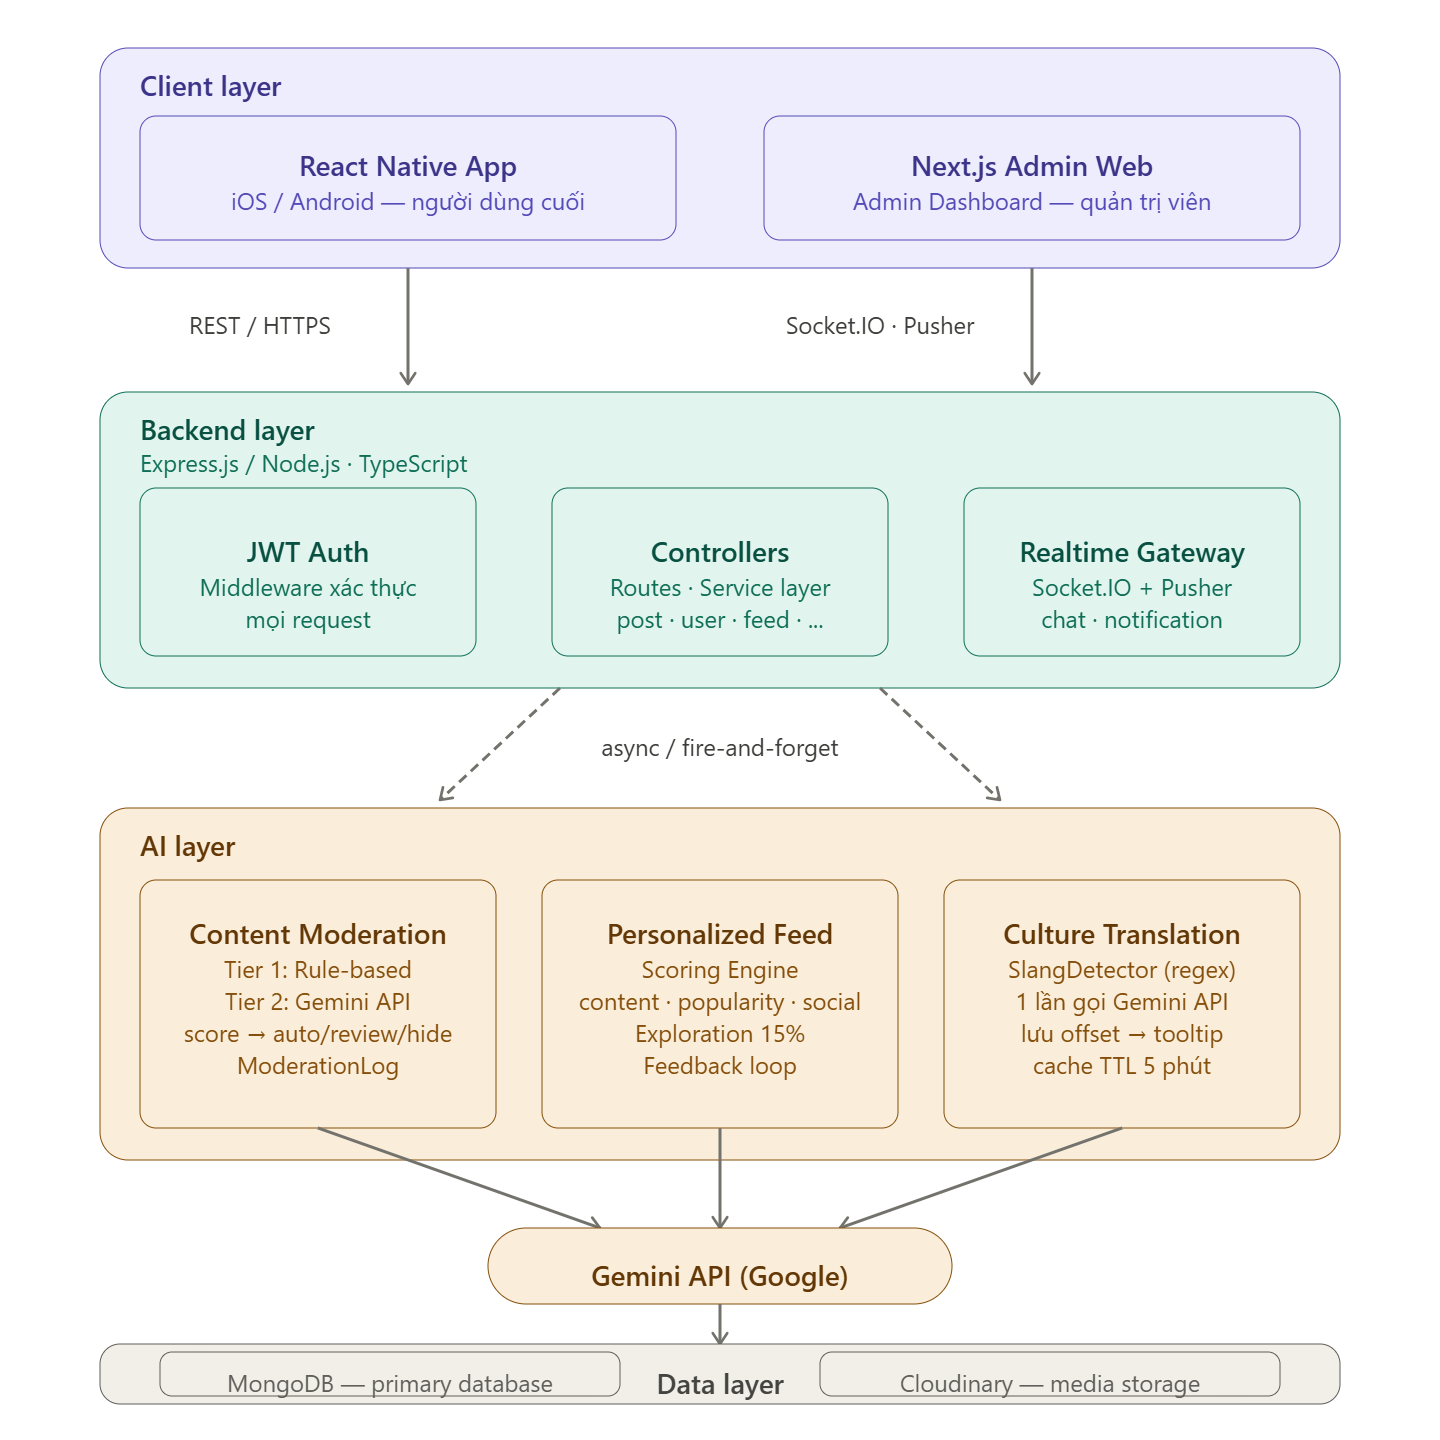
\includegraphics[width=\textwidth,height=0.72\textheight,keepaspectratio]{images/media/image10.png}
\caption{Kiến trúc tổng thể của hệ thống}
\caption*{\footnotesize Nguồn: Nhóm tác giả}
\end{figure}

\subsection{Module AI Content Moderation}

\textbf{Vấn đề và hướng tiếp cận}

Bài toán kiểm duyệt nội dung đặt ra hai yêu cầu cần cân bằng: tốc độ phản
hồi và khả năng phân tích ngữ cảnh. Mô hình ngôn ngữ có thể hỗ trợ xử lý
các trường hợp phụ thuộc ngữ nghĩa nhưng phát sinh độ trễ và chi phí khi
phải gọi API cho mọi nội dung. Trong khi đó, giải pháp thuần rule-based
lại có thể bỏ sót các vi phạm phụ thuộc ngữ cảnh. Hệ thống cân bằng hai
hướng tiếp cận bằng kiến trúc \textbf{2-Tier Pipeline}, kết hợp
rule-based filter và phân tích bằng mô hình ngôn ngữ.

{\def\LTcaptype{none} % do not increment counter
\begin{longtable}[]{@{}
  >{\centering\arraybackslash}p{(\linewidth - 8\tabcolsep) * \real{0.2505}}
  >{\centering\arraybackslash}p{(\linewidth - 8\tabcolsep) * \real{0.1965}}
  >{\centering\arraybackslash}p{(\linewidth - 8\tabcolsep) * \real{0.1812}}
  >{\centering\arraybackslash}p{(\linewidth - 8\tabcolsep) * \real{0.1568}}
  >{\centering\arraybackslash}p{(\linewidth - 8\tabcolsep) * \real{0.1568}}@{}}
\toprule\noalign{}
\endhead
\bottomrule\noalign{}
\endlastfoot
Phương án & Tốc độ & Chi phí & Khả năng phân tích ngữ cảnh & Phù hợp \\
Thuần Rule-based & Nhanh & Không phát sinh chi phí API & Hạn chế &
Không \\
Thuần LLM API & Phụ thuộc dịch vụ ngoài & Phát sinh theo số lần gọi &
Có & Không \\
2-Tier Hybrid & Có fast path & Giảm số lần gọi API & Kết hợp hai nguồn
tín hiệu & Phù hợp \\
\end{longtable}
}

\textbf{Tier 1 --- Rule-based Filter}

RuleBasedService thực hiện các phép kiểm tra đồng bộ bên trong tác vụ
kiểm duyệt. Tuy nhiên, khi tạo bài đăng, toàn bộ tác vụ kiểm duyệt được
khởi chạy sau khi bài viết đã được lưu và không được await trong request
chính. Module thực hiện ba lớp kiểm tra theo thứ tự ưu tiên, dừng lại và
trả kết quả ngay khi phát hiện vi phạm rõ ràng ở bất kỳ lớp nào.

\emph{Lớp 1 --- Profanity Blocklist:} Danh sách 100+ từ/cụm từ độc hại
(tiếng Việt và tiếng Anh) được pre-compiled tại thời điểm khởi động
thành BlocklistEntry với regex kèm word-boundary. Kỹ thuật word-boundary
(?:\^{}\textbar\textbackslash s)word(?:\textbackslash s\textbar\$) giải
quyết vấn đề false positive phổ biến khi từ vi phạm xuất hiện bên trong
một từ khác dài hơn --- ví dụ, từ "đụ" không được match nhầm trong
"đụng" hay "đụt". Văn bản đầu vào được chuẩn hóa trước (lowercase, bỏ
dấu NFD, thay dấu câu bằng khoảng trắng) để đảm bảo match nhất quán bất
kể cách viết của người dùng. Nếu khớp, hàm trả về isClearViolation =
true, score = 0.95.

\emph{Lớp 2 --- Hate-speech Pattern:} Bốn nhóm regex mô tả cấu trúc câu
thù hận đặc trưng trong tiếng Việt (đe dọa, miệt thị, kêu gọi bạo lực).
Mỗi regex được khởi tạo lại thông qua new RegExp(pattern.source,
pattern.flags) trước mỗi lần kiểm tra, thay vì tái sử dụng cùng một
object. Đây là biện pháp phòng tránh lỗi lastIndex --- một đặc tính của
JavaScript khi regex mang flag /g lưu trạng thái vị trí tìm kiếm giữa
các lần gọi .test(). Nếu tái sử dụng cùng một regex object, lần gọi thứ
ba hoặc thứ tư có thể trả về false trên cùng một chuỗi vi phạm, dẫn đến
bỏ sót nội dung độc hại một cách ngẫu nhiên. Nếu khớp, hàm trả về
isClearViolation = true, score = 0.92.

\emph{Lớp 3 --- Spam Signal:} Nếu nội dung vượt qua Lớp 1 và Lớp 2, hệ
thống tính điểm spam tổng hợp từ ba tín hiệu độc lập: ký tự lặp liên
tiếp từ 8 lần, nhiều link trong cùng một bài (≥ 2 URL), và toàn chữ hoa
trên đoạn văn dài (\textgreater{} 85\% uppercase trên \textgreater{} 40
ký tự). Khi có nhiều tín hiệu cùng xuất hiện, điểm được cộng dồn có giới
hạn theo công thức:

\emph{spamScore} = min(\emph{maxSignalScore} + 0.2 × (\emph{signalCount}
− 1), 0.9)

Kết quả Lớp 3 phân thành ba nhánh: spamScore ≥ 0.70 thì isClearViolation
= true --- chặn ngay; 0.25 ≤ spamScore \textless{} 0.70 thì needsAICheck
= true --- vùng nghi ngờ, chuyển sang Tier 2; spamScore \textless{} 0.25
--- nội dung sạch, duyệt ngay theo fast path.

\textbf{Tier 2 --- AI Moderation}

ModerationService nhận kết quả từ RuleBasedService và xử lý theo ba
nhánh chính. Nếu isClearViolation = true (từ bất kỳ lớp nào của Tier 1),
nội dung bị chặn ngay lập tức mà không gọi Gemini API. Nếu hàm
shouldCallAI() trả về true, hệ thống gọi Tier 2. Trường hợp còn lại, nội
dung được duyệt ngay theo fast path.

Tier 2 được kích hoạt khi thỏa một trong bốn điều kiện: needsAICheck =
true từ Lớp 3, nội dung bị người dùng báo cáo (reportCount
\textgreater{} 0), tài khoản mới (isNewAccount = true), hoặc lấy mẫu
ngẫu nhiên 5\% để kiểm soát chất lượng hệ thống. AIApiService gọi Gemini
API với prompt được thiết kế ép buộc mô hình trả về JSON chuẩn:

\{"toxic": number 0-1, "hate\_speech": number 0-1, "spam": number 0-1,
"reason": string\}

Sau khi nhận kết quả từ Gemini, hệ thống không dùng điểm AI thuần túy mà
tổng hợp với điểm từ Tier 1 bằng phép lấy MAX trên từng chiều đánh giá:

\emph{combinedToxic} = max(\emph{aiScores.toxic}, \emph{ruleScore} ×
0.35) \emph{combinedHateSpeech} = max(\emph{aiScores.hateSpeech},
\emph{ruleScore} × 0.3) \emph{combinedSpam} = max(\emph{aiScores.spam},
\emph{ruleScore})

Cơ chế này đảm bảo tín hiệu nghi ngờ từ Tier 1 không bị kết quả AI lạc
quan che khuất --- nếu rule-based đã thấy dấu hiệu spam (score = 0.4)
nhưng Gemini đánh giá sạch (spam = 0.1), điểm spam cuối cùng vẫn giữ
nguyên là 0.4. Quyết định cuối cùng dựa trên maxScore = max(toxic,
hateSpeech, spam) theo ngưỡng phân loại trong Bảng 3.3:

{\def\LTcaptype{none} % do not increment counter
\begin{longtable}[]{@{}
  >{\centering\arraybackslash}p{(\linewidth - 6\tabcolsep) * \real{0.1923}}
  >{\centering\arraybackslash}p{(\linewidth - 6\tabcolsep) * \real{0.2795}}
  >{\centering\arraybackslash}p{(\linewidth - 6\tabcolsep) * \real{0.1810}}
  >{\centering\arraybackslash}p{(\linewidth - 6\tabcolsep) * \real{0.3253}}@{}}
\toprule\noalign{}
\endhead
\bottomrule\noalign{}
\endlastfoot
maxScore & Quyết định & Trạng thái & Hành động \\
\textless{} 0.5 & Approved & APPROVED & Cho phép hiển thị \\
0.5 -- \textless{} 0.8 & Human Review & FLAGGED & Đưa vào danh sách cần xem xét \\
\textgreater{}= 0.8 & Auto Hide & REJECTED & Tự động ẩn, ghi
hiddenReason \\
\end{longtable}
}

\textbf{Cơ chế Fallback}

Hệ thống xử lý đầy đủ các trường hợp lỗi API (timeout, rate limit, JSON
parse error) theo nguyên tắc: bài đăng không bao giờ bị mất do lỗi AI.
Khi Gemini API thất bại do lỗi HTTP hoặc exception, AIApiService trả về
điểm mặc định thấp (toxic: 0.2, hateSpeech: 0, spam: 0.2) kèm lý do
fallback\_*. Với maxScore = 0.2 \textless{} 0.5, nội dung được phân loại
APPROVED theo ngưỡng hiện tại; thao tác tạo bài không bị trả lỗi. Trường
hợp parse JSON thất bại sử dụng bộ điểm fallback thấp hơn. Trạng thái và
các điểm kiểm duyệt được lưu trực tiếp trên document bài đăng hoặc bình
luận; các thao tác quản trị được ghi nhận qua cơ chế audit/log của hệ
thống.

Hình 3.2 mô tả luồng xử lý đầy đủ của 2-Tier Moderation Pipeline:

\begin{figure}[H]
\centering
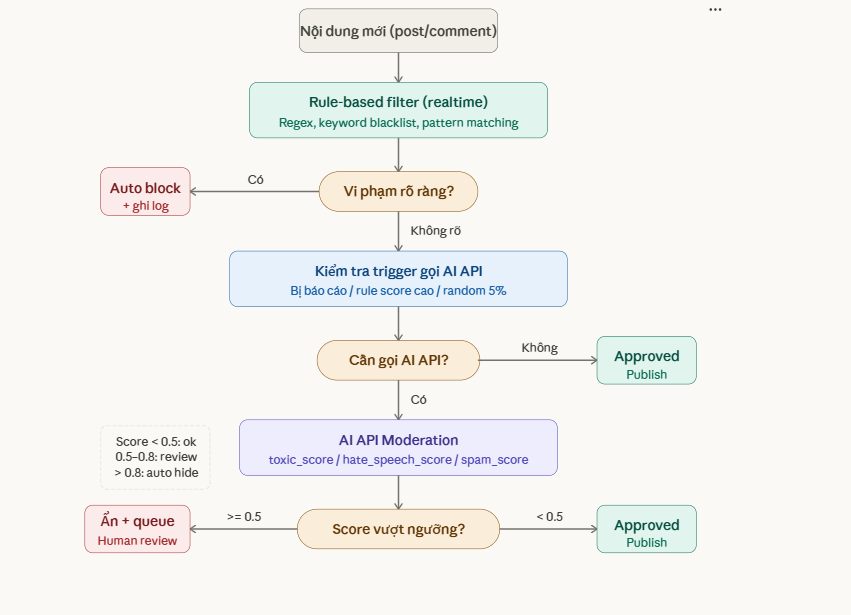
\includegraphics[width=\textwidth,height=0.68\textheight,keepaspectratio]{images/media/image9.png}
\caption{Luồng xử lý của 2-Tier Moderation Pipeline}
\caption*{\footnotesize Nguồn: Nhóm tác giả}
\end{figure}

\subsection{Module Personalized Feed}

\textbf{Vấn đề và hướng tiếp cận}

Hệ thống đề xuất nội dung thuần content-based filtering có xu hướng dẫn
đến "overspecialization" --- người dùng bị mắc kẹt trong vòng lặp nội
dung hẹp {[}9{]}. Hệ thống giải quyết vấn đề này bằng kiến trúc
\textbf{Hybrid Scoring} kết hợp ba chiều đánh giá độc lập (content,
popularity, social), bổ sung cơ chế Exploration chủ động đưa nội dung
ngoài vùng sở thích vào feed.

\textbf{Scoring Engine}

ScoringService tính điểm ranking cho mỗi bài đăng theo công thức tổng
hợp có trọng số:

\emph{finalScore} = \emph{w}₁ × \emph{contentScore} + \emph{w}₂ ×
\emph{popularityScore} + \emph{w}₃ × \emph{socialScore}

Trọng số được điều chỉnh tự động dựa trên lượng dữ liệu hành vi của
người dùng, phân biệt hai chế độ theo Bảng 3.9:

Bảng 3.9: Trọng số Scoring Engine theo chế độ người dùng
\addcontentsline{lot}{table}{\protect\numberline{3.9}Trọng số Scoring Engine theo chế độ người dùng}

{\def\LTcaptype{none} % do not increment counter
\begin{longtable}[]{@{}
  >{\centering\arraybackslash}p{(\linewidth - 6\tabcolsep) * \real{0.1923}}
  >{\centering\arraybackslash}p{(\linewidth - 6\tabcolsep) * \real{0.2795}}
  >{\centering\arraybackslash}p{(\linewidth - 6\tabcolsep) * \real{0.1810}}
  >{\centering\arraybackslash}p{(\linewidth - 6\tabcolsep) * \real{0.3253}}@{}}
\toprule\noalign{}
\endhead
\bottomrule\noalign{}
\endlastfoot
Thành phần & Normal (\textgreater= 10 tương tác) & Cold Start
(\textless{} 10 tương tác) & Lý do \\
Content (\emph{w}₁) & 0.50 & 0.05 & Người dùng mới chưa có đủ profile \\
Popularity (\emph{w}₂) & 0.20 & 0.7 & Nội dung phổ biến phù hợp khi
thiếu dữ liệu \\
Social (\emph{w}₃) & 0.30 & 0.25 & Ưu tiên người đang follow \\
\end{longtable}
}

\emph{Content Score} đo độ khớp giữa bài đăng và UserProfile của người
dùng. TopicExtractorService trích xuất tối đa 3 chủ đề từ bài đăng bằng
cách tính điểm keyword matching trên hai tầng: hashtag (trọng số ×2) và
từ khóa trong nội dung (trọng số ×1), đối chiếu với từ điển
social\_media\_topics\_v2.json gồm các chủ đề tiếng Việt lẫn tiếng Anh.
Content Score được tính:

\emph{contentScore} = Σ \emph{topicScores}{[}topic{]} +
\emph{authorScores}{[}authorId{]} × 1.2

\emph{Popularity Score} sử dụng trường hotScore đã được tính sẵn bởi
cron job định kỳ 30 phút. Khi hotScore chưa có, hệ thống tính tạm theo
công thức có tham số gravity kiểm soát tốc độ suy giảm theo thời gian:

\emph{rawPopularity} = \emph{engagements} / (\emph{ageHours} +
2)\^{}\emph{gravity}

\emph{popularityScore} = min(\emph{rawPopularity} × 2, 100)

Trong đó \emph{gravity} = 1.5 và:

\emph{engagements} = likes × 3 + comments × 4 + shares × 5 + saves × 4 +
views × 0.1

\emph{Social Score} nhị phân: bài đăng từ tác giả đang được follow nhận
điểm tối đa (100), ngược lại nhận 0. Tính đơn giản nhưng hiệu quả trong
việc ưu tiên nội dung từ mạng lưới gần.

\textbf{Exploration}

Để tránh filter bubble, 15\% số lượng bài đăng trong feed
(\texttt{EXPLORATION\_\allowbreak RATE} = 0.15) được chọn từ pool ứng viên ngoài vùng sở
thích hiện tại, đảm bảo người dùng tiếp xúc với nội dung đa dạng ngay cả
khi hệ thống đã hội tụ về sở thích hẹp.

\textbf{Feedback Loop}

InteractionTrackerService thu thập tín hiệu hành vi người dùng và cập
nhật liên tục vào UserProfile. Mỗi loại tương tác mang trọng số và hệ số
decay khác nhau theo Bảng 3.10:

Bảng 3.10: Trọng số và hệ số decay theo loại tương tác
\addcontentsline{lot}{table}{\protect\numberline{3.10}Trọng số và hệ số decay theo loại tương tác}

{\def\LTcaptype{none} % do not increment counter
\begin{longtable}[]{@{}
  >{\centering\arraybackslash}p{(\linewidth - 6\tabcolsep) * \real{0.2282}}
  >{\centering\arraybackslash}p{(\linewidth - 6\tabcolsep) * \real{0.2672}}
  >{\centering\arraybackslash}p{(\linewidth - 6\tabcolsep) * \real{0.1744}}
  >{\centering\arraybackslash}p{(\linewidth - 6\tabcolsep) * \real{0.3084}}@{}}
\toprule\noalign{}
\endhead
\bottomrule\noalign{}
\endlastfoot
Loại tương tác & Trọng số (weight) & Decay & Ý nghĩa \\
follow\_\allowbreak from\_\allowbreak post & 6 & 1.2 & Tín hiệu mạnh nhất --- chủ động theo
dõi \\
share & 5 & 1.0 & Muốn lan truyền nội dung \\
comment & 4 & 1.0 & Tương tác sâu \\
save & 4 & 1.0 & Muốn xem lại \\
like & 3 & 1.0 & Thích nội dung \\
see\_more & 2 & 0.8 & Muốn xem thêm về chủ đề \\
view & 1 & 0.6 & Tín hiệu yếu --- có thể vô tình \\
not\_interested & -3 & 1.0 & Phản hồi tiêu cực nhẹ \\
hide & -5 & 1.0 & Phản hồi tiêu cực mạnh \\
\end{longtable}
}

Delta cập nhật vào UserProfile được tính:

\emph{delta} = \emph{weight} × \emph{decay}

Cập nhật áp dụng cho topicScores (delta × 1.0), hashtagScores (delta ×
0.9) và authorScores (delta × 0.7) của người dùng. Toàn bộ dữ liệu tương
tác được lưu trong UserInteraction với TTL index tự động xóa sau 90
ngày, đảm bảo UserProfile phản ánh sở thích hiện tại thay vì lịch sử quá
xa.

Hình 3.3 mô tả pipeline đầy đủ của Personalized Feed:

\begin{figure}[H]
\centering
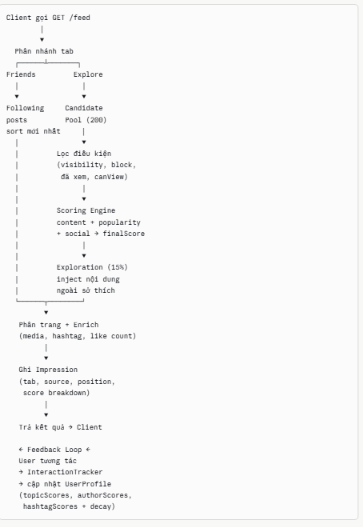
\includegraphics[width=0.62\textwidth,height=0.68\textheight,keepaspectratio]{images/media/image6.png}
\caption{Luồng xử lý của Personalized Feed}
\caption*{\footnotesize Nguồn: Nhóm tác giả}
\end{figure}

\subsection{Module giải thích thuật ngữ và ngữ cảnh văn hóa mạng}

\textbf{Vấn đề và hướng tiếp cận}

Ngôn ngữ mạng (slang, meme, internet culture reference) phát triển nhanh
chóng tạo ra rào cản giao tiếp giữa các thế hệ và nhóm văn hóa. Các nền
tảng hiện tại chưa có cơ chế giải thích ngữ cảnh văn hóa, dẫn đến hiểu
nhầm và giảm khả năng tiếp cận của người dùng lớn tuổi {[}6{]}. Phương
án gọi LLM mỗi khi người dùng hover vào từ sẽ gây độ trễ cao và chi phí
không kiểm soát được. Hệ thống giải quyết bằng chiến lược \textbf{phân
tích một lần tại thời điểm đăng bài} --- kết quả được lưu vào MongoDB và
phục vụ trực tiếp từ database khi người đọc tương tác.

\textbf{Pipeline xử lý}

Toàn bộ pipeline chạy bất đồng bộ (fire-and-forget) sau khi bài đăng đã
được lưu thành công, không chặn luồng phản hồi của người dùng.

\emph{Bước 1 --- Rule-based Detection (SlangDetectorService):}
SlangDetectorService tải từ điển slang từ SlangEntryModel trong MongoDB
với cơ chế in-memory cache TTL 5 phút, tránh truy vấn DB lặp lại cho mỗi
bài đăng. Với mỗi entry trong từ điển, regex được build từ trường
regexPattern lưu trong DB và thực thi với flag /gi để tìm tất cả vị trí
xuất hiện trong nội dung. Kết quả trả về danh sách DetectedTerm kèm vị
trí ký tự chính xác (startIndex, endIndex) --- dữ liệu cần thiết để
frontend highlight đúng vị trí trong chuỗi gốc. Bước này hoàn toàn không
tốn chi phí API.

\emph{Bước 2 --- Một lần gọi LLM (CultureLLMService):} Thay vì gọi API
riêng lẻ cho từng thuật ngữ, toàn bộ danh sách thuật ngữ phát hiện được
gộp vào \textbf{một lần gọi Gemini API duy nhất}. Đây là điểm tối ưu chi
phí quan trọng nhất của module --- giả sử một bài đăng chứa 5 thuật ngữ
slang, phương án gọi riêng lẻ tốn 5 lần API, phương án batch chỉ tốn 1
lần.

Prompt được thiết kế cung cấp ngữ cảnh bài viết (300 ký tự đầu) để LLM
giải thích đúng nghĩa trong văn cảnh cụ thể, không chỉ nghĩa từ điển
chung. Đầu ra yêu cầu JSON array chuẩn, mỗi phần tử gồm: term, meaning
(giải thích tối đa 2 câu), origin (TikTok / Reddit VN / Gaming / Twitter
/ Chung), tone (tích cực / trung tính / hài hước / tiêu cực),
contextNote (cách dùng trong bài này). Tương tự module Moderation, mọi
trường hợp lỗi API đều có fallback trả về cấu trúc rỗng, không làm crash
pipeline.

\emph{Bước 3 --- Merge và lưu MongoDB:} Kết quả giải thích từ LLM được
ghép với vị trí ký tự từ Bước 1 thông qua explainMap (Map theo term
lowercase). Dữ liệu culturalTerms được lưu trực tiếp vào document bài
đăng kèm cờ cultureAnalyzed = true để tránh xử lý lại.

\emph{Bước 4 --- Hiển thị Tooltip (Frontend):} Khi người đọc mở bài
đăng, client nhận culturalTerms kèm startIndex/endIndex, tự động
highlight các thuật ngữ trong văn bản. Người dùng nhấn vào thuật ngữ
được highlight sẽ thấy tooltip giải thích từ dữ liệu đã lưu --- không
phát sinh thêm lần gọi Gemini API. Cách tiếp cận này loại bỏ độ trễ gọi
LLM tại thời điểm người đọc mở phần giải thích, dù thời gian hiển thị
thực tế vẫn phụ thuộc vào mạng và quá trình tải dữ liệu từ backend.

\textbf{Xử lý khi chỉnh sửa bài}

Khi tác giả chỉnh sửa nội dung, reAnalyzePost reset culturalTerms về
mảng rỗng và cultureAnalyzed về false, sau đó gọi lại toàn bộ pipeline
bất đồng bộ. Cơ chế này đảm bảo kết quả phân tích luôn khớp với nội dung
hiện tại của bài đăng.

Hình 3.4 mô tả luồng xử lý của Culture Translation Pipeline:

\begin{figure}[H]
\centering
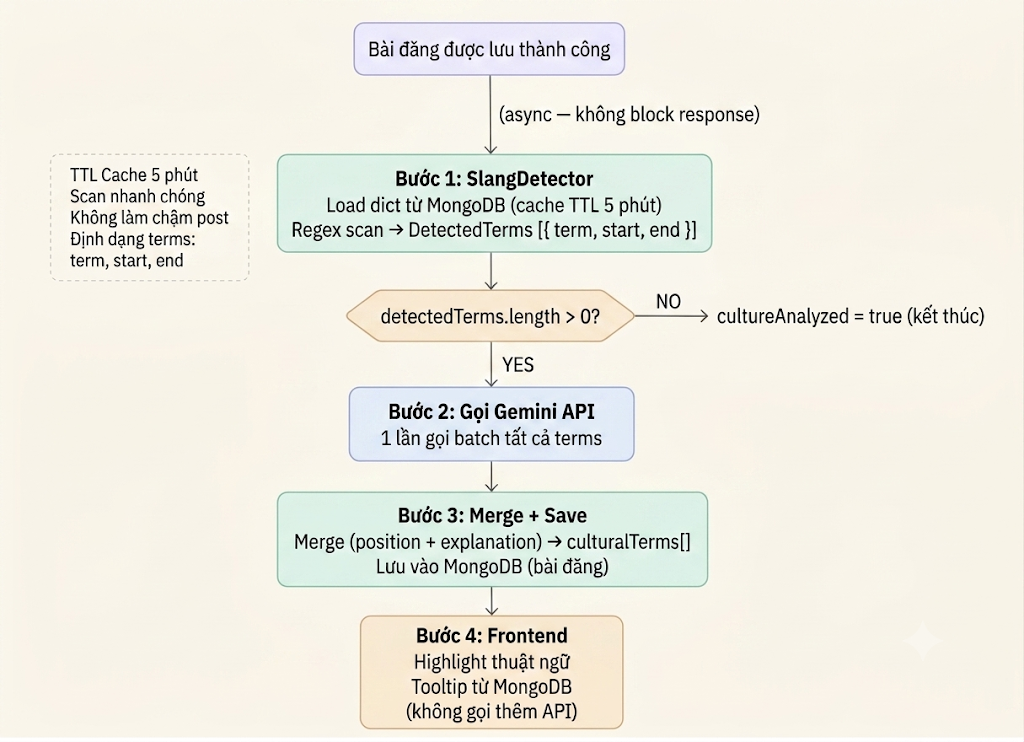
\includegraphics[width=\textwidth,height=0.68\textheight,keepaspectratio]{images/media/image11.png}
\caption{Luồng giải thích thuật ngữ và ngữ cảnh văn hóa mạng}
\caption*{\footnotesize Nguồn: Nhóm tác giả}
\end{figure}

\section{Thiết kế Use Case}

\subsection{Danh sách các Actor}

\subsection{Danh sách các Use Case chính}

\subsection{Đặc tả chi tiết Use Case}

\textit{Phần này sẽ được bổ sung các use case quan trọng sau khi hoàn
thiện tài liệu phân tích.}

\section{Sơ đồ Activity}

\textit{Phần này sẽ được bổ sung các sơ đồ Activity của các chức năng
chính.}

\section{Thiết kế dữ liệu}

\subsection{Sơ đồ lớp (Class Diagram)}

\subsection{Sơ đồ ERD}

\subsection{Mô tả chi tiết các collection}

\textit{Phần này sẽ được bổ sung sau khi hoàn thiện sơ đồ ERD và bảng mô
tả dữ liệu.}

\chapter{XÂY DỰNG ỨNG DỤNG}

Chương này trình bày giao diện của ứng dụng di động, trang quản trị và
các kết quả tích hợp module hỗ trợ thông minh. Khi hoàn thiện bản Word,
mỗi ảnh cần được chèn bằng chức năng \textbf{References → Insert Caption},
đặt nhãn ``Hình'', đánh số theo chương và ghi nguồn ``Nhóm tác giả'' nếu
ảnh do nhóm tự chụp.

\section{Giao diện ứng dụng di động}

Các hình nên được chụp cùng một thiết bị hoặc khung giả lập, có kích
thước thống nhất và che thông tin nhạy cảm. Danh sách hình đề xuất:

{\def\LTcaptype{none}
\begin{longtable}[]{@{}
  >{\centering\arraybackslash}p{0.12\linewidth}
  >{\raggedright\arraybackslash}p{0.32\linewidth}
  >{\raggedright\arraybackslash}p{0.50\linewidth}@{}}
\toprule\noalign{}
\textbf{Số hình} & \textbf{Màn hình cần chụp} & \textbf{Chú thích đề xuất} \\
\midrule\noalign{}
\endhead
\bottomrule\noalign{}
\endlastfoot
Hình 4.1 & Đăng nhập & Giao diện đăng nhập bằng email hoặc số điện thoại \\
Hình 4.2 & Đăng ký & Giao diện đăng ký tài khoản người dùng \\
Hình 4.3 & Xác thực tài khoản & Giao diện xác thực email hoặc số điện thoại bằng mã OTP \\
Hình 4.4 & Xác thực hai yếu tố & Giao diện thiết lập và xác nhận mã xác thực hai yếu tố \\
Hình 4.5 & Feed Khám phá & Giao diện feed Khám phá với nội dung được xếp hạng cá nhân hóa \\
Hình 4.6 & Feed Bạn bè & Giao diện feed hiển thị bài viết từ các tài khoản đang theo dõi \\
Hình 4.7 & Tạo bài viết & Giao diện tạo bài viết gồm văn bản, hashtag, mention và quyền riêng tư \\
Hình 4.8 & Chi tiết bài viết & Giao diện chi tiết bài viết và các thông tin tương tác \\
Hình 4.9 & Bình luận & Giao diện danh sách bình luận và trả lời bình luận \\
Hình 4.10 & Tìm kiếm & Giao diện tìm kiếm người dùng, bài viết và hashtag \\
Hình 4.11 & Hồ sơ cá nhân & Giao diện hồ sơ cá nhân và danh sách bài viết của người dùng \\
Hình 4.12 & Quan hệ người dùng & Giao diện danh sách người theo dõi, đang theo dõi và bạn thân \\
Hình 4.13 & Bài viết đã lưu & Giao diện quản lý các bài viết người dùng đã lưu \\
Hình 4.14 & Thông báo & Giao diện danh sách thông báo của người dùng \\
Hình 4.15 & Danh sách trò chuyện & Giao diện danh sách cuộc trò chuyện gần đây \\
Hình 4.16 & Chi tiết trò chuyện & Giao diện nhắn tin trực tiếp hoặc trò chuyện nhóm \\
Hình 4.17 & Cuộc gọi & Giao diện cuộc gọi thời gian thực sử dụng WebRTC \\
Hình 4.18 & Báo cáo nội dung & Giao diện gửi báo cáo đối với bài viết, bình luận hoặc tài khoản \\
\end{longtable}
}

\section{Giao diện trang quản trị}

Các ảnh trang quản trị nên chụp trên cùng kích thước cửa sổ trình duyệt,
ưu tiên hiển thị đầy đủ thanh điều hướng và vùng nội dung chính.

{\def\LTcaptype{none}
\begin{longtable}[]{@{}
  >{\centering\arraybackslash}p{0.12\linewidth}
  >{\raggedright\arraybackslash}p{0.32\linewidth}
  >{\raggedright\arraybackslash}p{0.50\linewidth}@{}}
\toprule\noalign{}
\textbf{Số hình} & \textbf{Màn hình cần chụp} & \textbf{Chú thích đề xuất} \\
\midrule\noalign{}
\endhead
\bottomrule\noalign{}
\endlastfoot
Hình 4.19 & Đăng nhập quản trị & Giao diện đăng nhập dành cho quản trị viên \\
Hình 4.20 & Dashboard & Giao diện tổng quan số liệu người dùng, nội dung và báo cáo \\
Hình 4.21 & Quản lý người dùng & Giao diện danh sách và tìm kiếm tài khoản người dùng \\
Hình 4.22 & Chi tiết người dùng & Giao diện xem thông tin, thống kê và trạng thái tài khoản \\
Hình 4.23 & Quản lý bài viết & Giao diện danh sách bài viết và trạng thái kiểm duyệt \\
Hình 4.24 & Chi tiết bài viết & Giao diện xem nội dung, điểm kiểm duyệt và lịch sử xử lý bài viết \\
Hình 4.25 & Quản lý bình luận & Giao diện danh sách và xử lý bình luận \\
Hình 4.26 & Danh sách báo cáo & Giao diện tổng hợp các báo cáo đang chờ xử lý \\
Hình 4.27 & Chi tiết báo cáo & Giao diện xem thông tin báo cáo và thực hiện hành động quản trị \\
Hình 4.28 & Hiệu suất AI & Giao diện thống kê điểm và kết quả kiểm duyệt nội dung \\
Hình 4.29 & Nhật ký hệ thống & Giao diện theo dõi audit log và hoạt động quản trị \\
Hình 4.30 & Từ điển tiếng lóng & Giao diện quản lý từ điển thuật ngữ văn hóa mạng \\
\end{longtable}
}

\section{Minh họa các module hỗ trợ thông minh}

Nhóm hình này nên sử dụng cùng một dữ liệu mẫu trước và sau xử lý để làm
rõ đầu vào, kết quả và giá trị của từng module.

{\def\LTcaptype{none}
\begin{longtable}[]{@{}
  >{\centering\arraybackslash}p{0.12\linewidth}
  >{\raggedright\arraybackslash}p{0.32\linewidth}
  >{\raggedright\arraybackslash}p{0.50\linewidth}@{}}
\toprule\noalign{}
\textbf{Số hình} & \textbf{Nội dung cần chụp} & \textbf{Chú thích đề xuất} \\
\midrule\noalign{}
\endhead
\bottomrule\noalign{}
\endlastfoot
Hình 4.31 & Kiểm duyệt nội dung & Kết quả phân loại và các điểm toxic, hate-speech, spam của một bài viết mẫu \\
Hình 4.32 & Nội dung bị gắn cờ hoặc ẩn & Trạng thái hiển thị của nội dung sau khi vượt ngưỡng kiểm duyệt \\
Hình 4.33 & Cá nhân hóa feed & Kết quả xếp hạng feed kèm các thành phần content, popularity và social score \\
Hình 4.34 & Giải thích thuật ngữ & Giao diện làm nổi bật thuật ngữ văn hóa mạng và hiển thị phần giải thích theo ngữ cảnh \\
\end{longtable}
}

\section{Liên kết mã nguồn}

Phần này cần cung cấp liên kết tới repository backend, ứng dụng di động
và trang quản trị; đồng thời ghi rõ commit hoặc phiên bản được sử dụng
để xây dựng bản báo cáo. Không đưa khóa API, mật khẩu hoặc tập tin môi
trường vào repository công khai.

\chapter*{TÀI LIỆU THAM KHẢO}
\addcontentsline{toc}{chapter}{TÀI LIỆU THAM KHẢO}
\sloppy

{[}1{]} DataReportal \& Manochi, "Global Social Media Statistics," Apr.
2026. {[}Online{]}. Available:
\url{https://datareportal.com/social-media-users}

{[}2{]} Statista, DataReportal, and We Are Social, "Number of internet
and social media users worldwide," Oct. 2025. {[}Online{]}. Available:
\url{https://www.statista.com/statistics/617136/digital-population-worldwide/}

{[}3{]} EMARKETER, "Meta\textquotesingle s content moderation pullback
cuts takedown errors, removals," May 2025. {[}Online{]}. Available:
\url{https://www.emarketer.com/content/meta-content-moderation-pullback-cuts-takedown-errors-removals}

{[}4{]} Statista, "Meta\textquotesingle s Hate Speech Problem --- Hate
speech on social media," 2024. {[}Online{]}. Available:
\url{https://www.statista.com/chart/amp/21704/hate-speech-content-removed-by-facebook}

{[}5{]} GLAAD, "Make Meta Safe: New Report Finds Increase in Harmful
Content," June 2025. {[}Online{]}. Available:
\url{https://glaad.org/make-meta-safe-new-report/}

{[}6{]} Center for Democracy and Technology, "Intersectional Disparities
within Automated Hate-speech Detection," 2025. {[}Online{]}. Available:
\url{https://cdt.org/insights/intersectional-disparities-within-automated-hate-speech-detection/}

{[}7{]} Springer Nature, "LLM synthetic generation to enhance online
content moderation generalization," \emph{Journal of Supercomputing},
2025. {[}Online{]}. Available:
\url{https://link.springer.com/article/10.1007/s00607-025-01518-8}

{[}8{]} MDPI Social Sciences, "Trap of Social Media Algorithms: A
Systematic Review on Filter Bubbles, Echo Chambers, and Their Impact on
Youth," \emph{Social Sciences}, vol. 14, no. 11, p. 301, 2025.
{[}Online{]}. Available:
\url{https://www.mdpi.com/2075-4698/15/11/301}

{[}9{]} OurMental.Health, "How TikTok\textquotesingle s Algorithm
Creates Filter Bubbles and Amplifies Biases," Dec. 2024. {[}Online{]}.
Available:
\url{https://www.ourmental.health/screen-time-sanity/how-tiktoks-algorithm-shapes-user-perceptions}

{[}10{]} Morningstar Sustainalytics, "Meta\textquotesingle s Content
Moderation Overhaul: Key Risk Considerations," 2025. {[}Online{]}.
Available:
\href{https://www.sustainalytics.com/esg-research/resource/investors-esg-blog/meta-s-content-moderation-overhaul}{sustainalytics.com -- Meta's Content Moderation Overhaul}
\fussy
